\section{Experimental results and discussions}
\label{sec:experimental_results}
In order to show the accuracy of the proposed model of EM reliability for multi-branch interconnect three with line structure shown in Fig. \ref{fig:interconnect_tree}, the analytical solution \eqref{eq:general_solution} of stress evolution equations is calculated with the MATLAB enviroment, and we also compare the results from \eqref{eq:general_solution} with those obtained by the finite element tool COMSOL \cite{?}. In our experiments, we test three cases of interconnect tree structure by changing $n$ in \eqref{eq:general_solution} which is the number of wire segments in the interconnect tree. In the simulations to be described below, the following parameter values will be used: $Z^*=10$, $\rho=3\times10^{-8} \Omega/m$, $\Omega=8.78\times10^{-30}m^3$, $B=5.5\times10^{10} Pa$, $D_0=5.5\times10^{-5} m^2/s$, $E_a=1.1eV$, $e=1.6\times10^{-19}C$, $k=1.38\times10^{-23}J/K$ , and $T=350K$.

\subsection{Four-terminal interconnect wire ($n=3$)}
\begin{figure}[!h]
\centering
\subfigure[]{
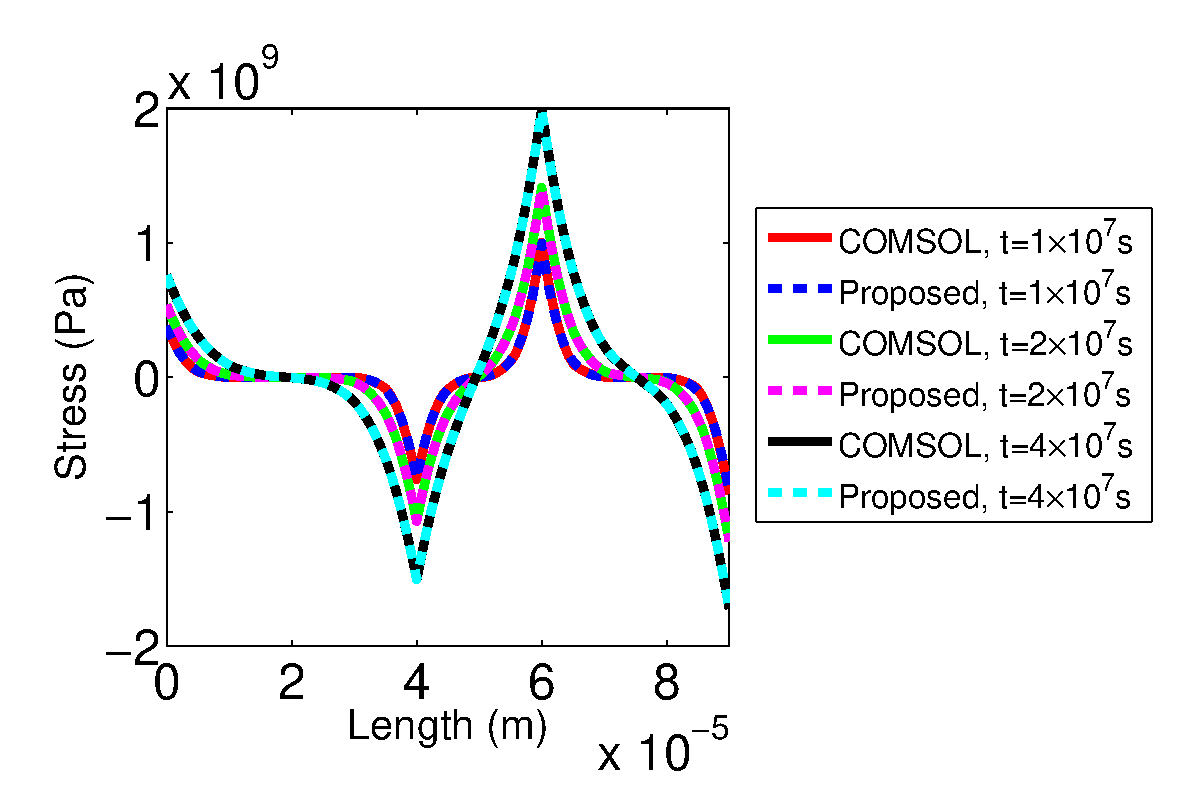
\includegraphics[width=0.9\columnwidth]{S3StressMatComCompareT0.eps}
\label{fig:ST3Compare}}
\subfigure[]{
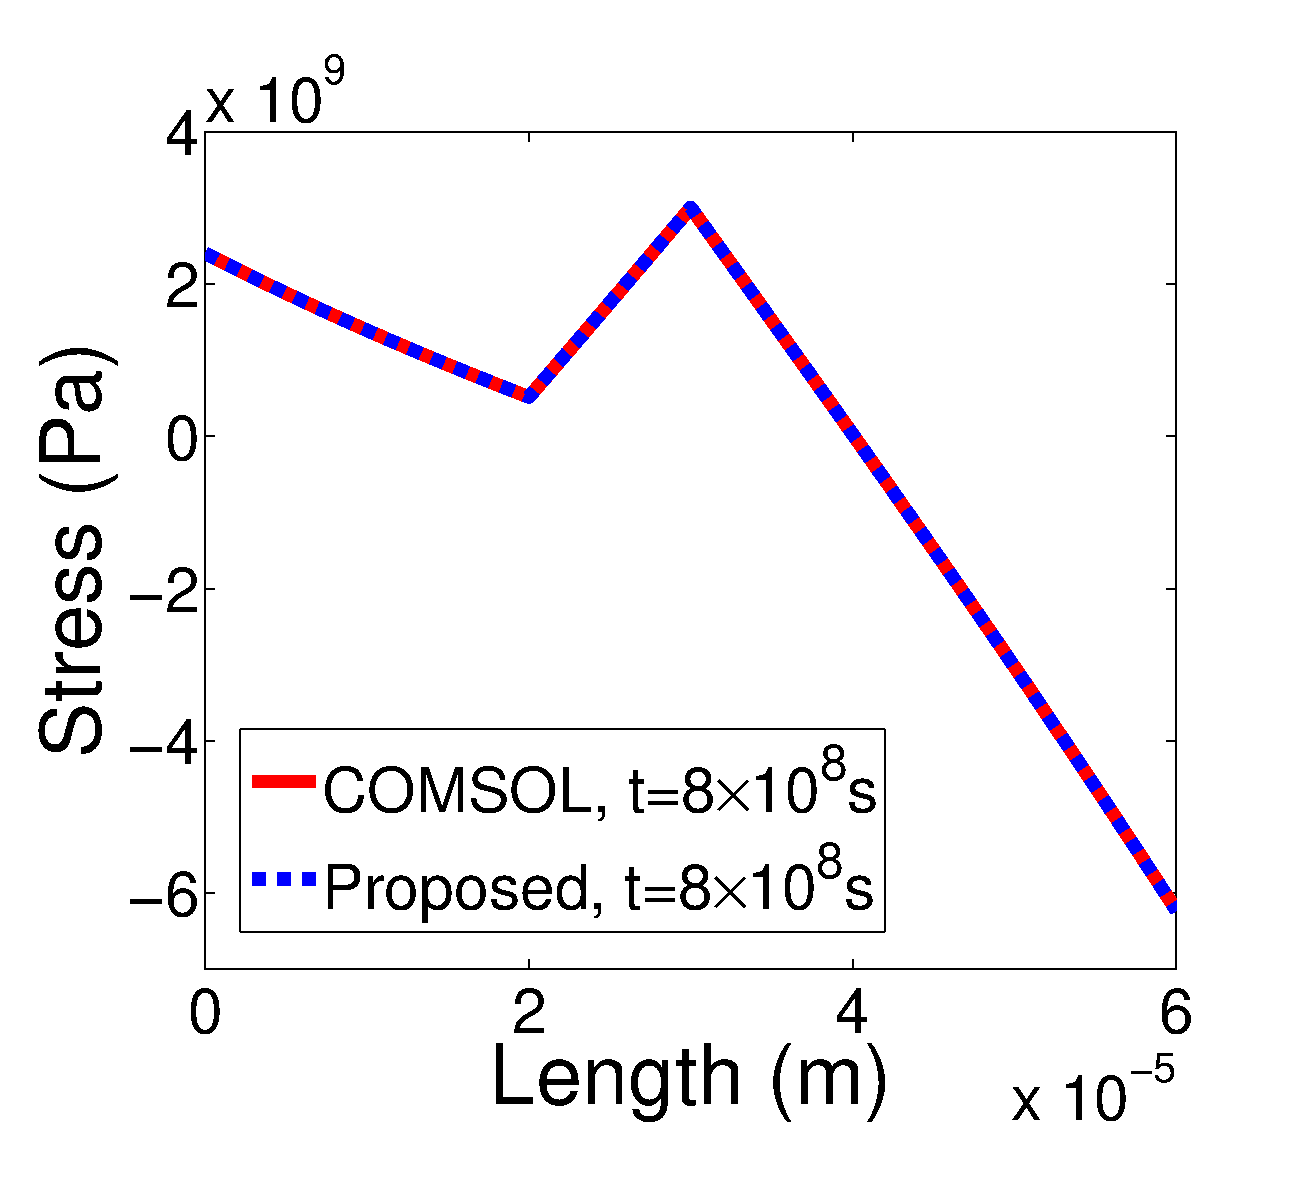
\includegraphics[width=0.6\columnwidth]{S3StableT0.eps}
\label{fig:ST3Stable}}
\caption{The experiments results of straight line at changing temperatures, $j_1=2\times10^{10}A/m^2,\;j_2=6\times10^{10}A/m^2$ (a) the comparison of stress evolution at square wave temperature at a fixed time; (b) the comparison of stress evolution at sine wave temperature at a fixed time; (c) the comparison of stress evolution at square wave temperature at a fixed position; (d) the comparison of stress evolution at sine wave temperature at a fixed position}
\label{fig:S3Results1}
\end{figure}


\begin{figure}[!h]
\centering
\subfigure[]{
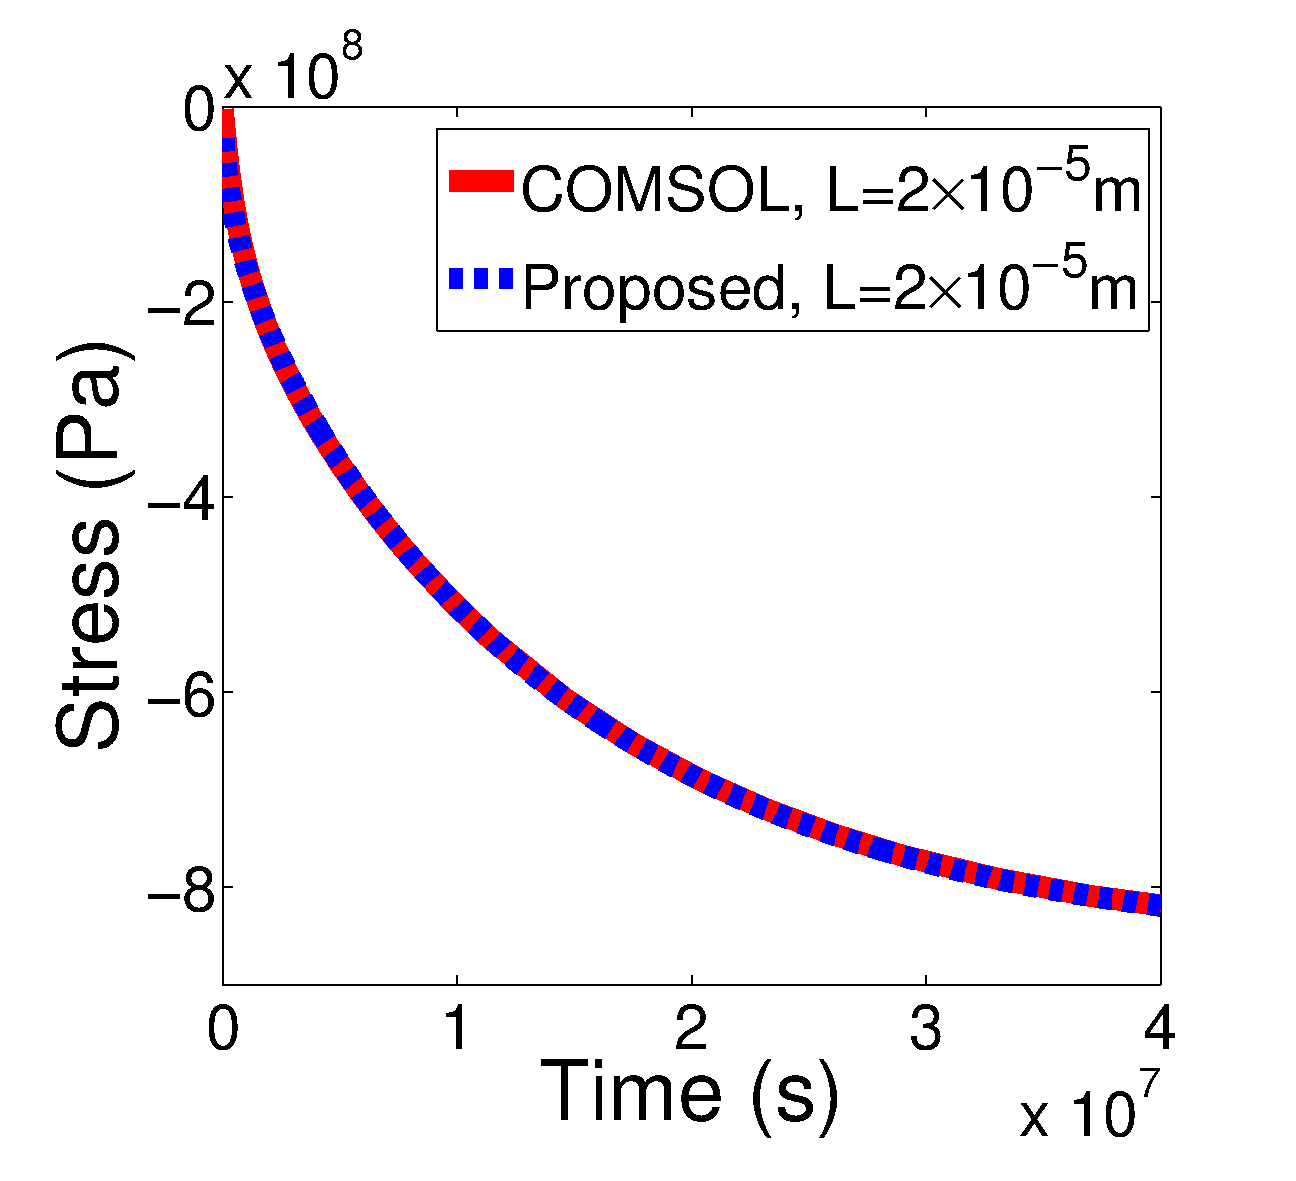
\includegraphics[width=0.45\columnwidth]{S3LengthCompare2T0.eps}
\label{fig:S3point1}}
\subfigure[]{
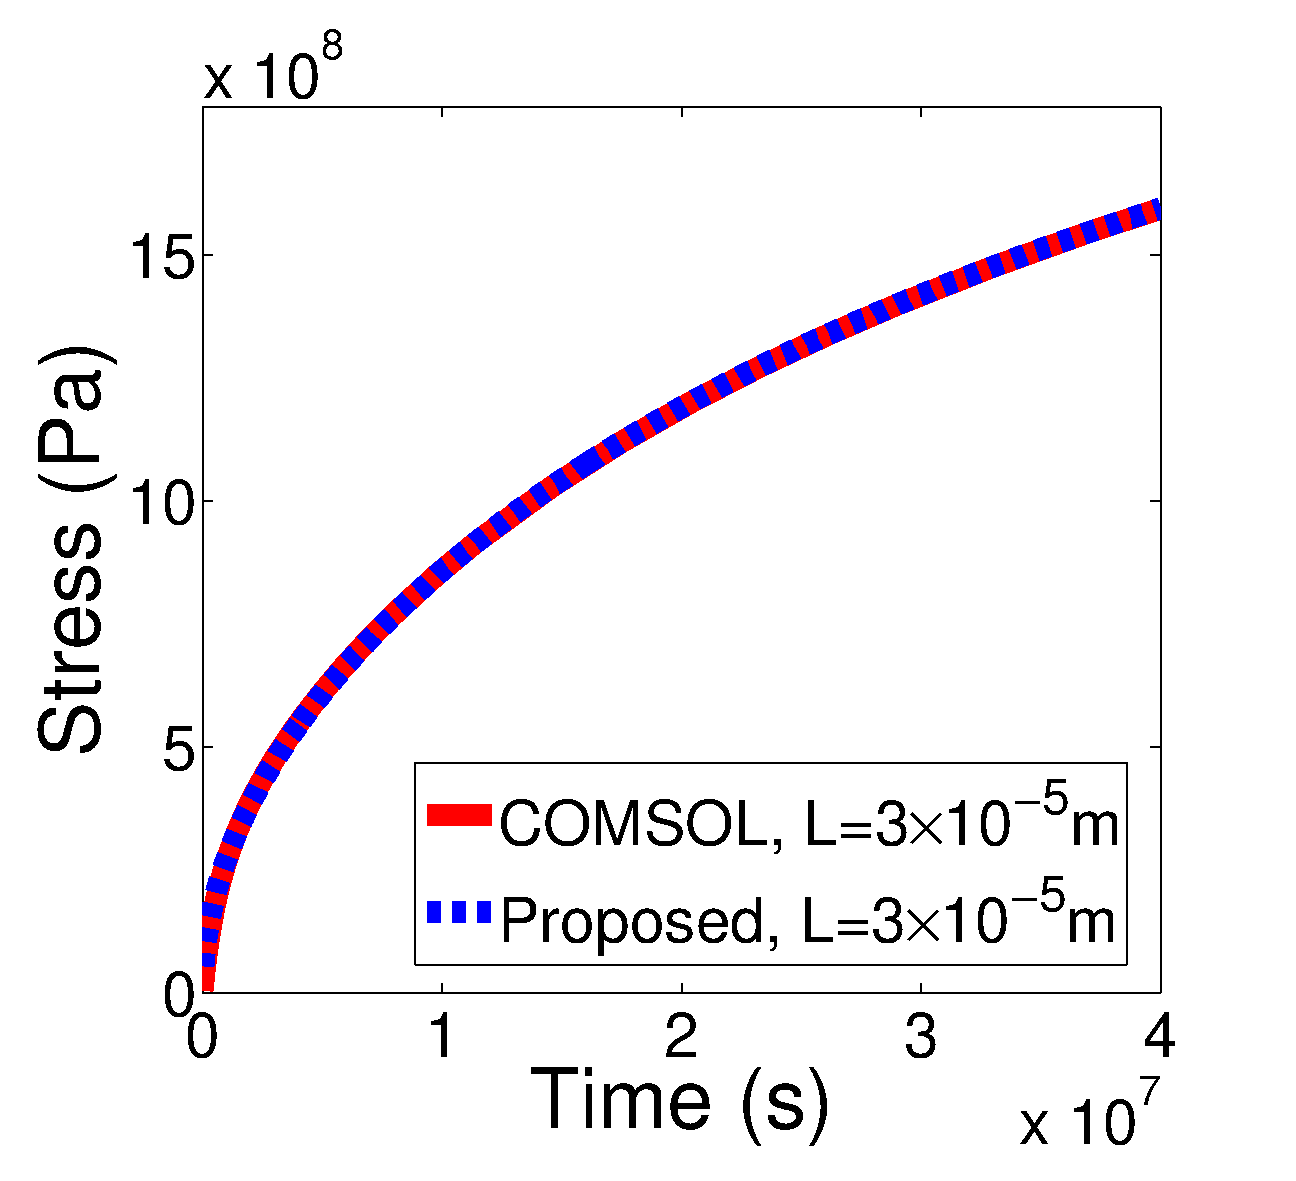
\includegraphics[width=0.45\columnwidth]{S3LengthCompare3T0.eps}
\label{fig:S3point2}}
\caption{The experiments results of straight line at changing temperatures, $j_1=2\times10^{10}A/m^2,\;j_2=6\times10^{10}A/m^2$ (a) the comparison of stress evolution at square wave temperature at a fixed time; (b) the comparison of stress evolution at sine wave temperature at a fixed time; (c) the comparison of stress evolution at square wave temperature at a fixed position; (d) the comparison of stress evolution at sine wave temperature at a fixed position}
\label{fig:S3Results2}
\end{figure}

We first analyze the four-terminal interconnect tree with three wire segments with the current flow directions as shown in Fig. \cite{}. A constant current density of $j_1=??$ is applied in the left segment, $j_2=$ is used to stress the middle wire segment, and $j_3=$ represent the current density of the right wire segment. The lengths for each wire segment in this interconnect tree are set to be $?m$, $?m$, and $?m$, respectively.


%Fig. were used in tests of the dotted-I structures. A constant
%current density of j1 = 2.5 MA/cm2 was applied in the left
%segment, while a current density with varying direction and
%magnitude, j2, was used to stress the right limb (segment).
%The distribution of the times-to-failure, TTFs, of the dotted-I
%structures is plotted on a lognormal scale in Figure 2(b).
%Failure was defined as the minimum time needed for a 30%
%increase in the resistance in either one of the segments in the
%test structure.

We first analyze the 3-terminal interconnect tree with two segments with the current flow directions as showed in Fig.\ref{fig:singleline}. Fig.\ref{fig:SResults} shows obtained evolution of the stress distribution. From Fig.\ref{fig:ST1Compare} and Fig.\ref{fig:ST2Compare}, analytical solution obtained with the proposed method fits well to the results of the numerical simulation at every time instance. For a fixed position shown in Fig.\ref{fig:ST1Length} and Fig.\ref{fig:ST2Length}, the stress changes in agreement with the varying temperatures. In the case of square ware temperature, when temperature rises up to $380K$, the stress is going through dramatic changes. On the contrary, when temperature is $320K$, the stress is smoothly continuous. In the case of sine wave temperature, when temperature falls down to below $250K$, the stress has a process of slow change. And average temperature is useless for the interconnect tree analysis. Thermal effects depended on the varying temperature are remarkable.

We first apply the COMSOL to compute an accurate numerical solution of \eqref{eq:basic_em}. We set the width of 3D interconnect tree as $10^{-8}m$, considering the thin and narrow interconnect line. Then we use the proposed approach to estimate the stress in MATLAB. Comparisons are shown in Fig.~\ref{fig:SResults}, Fig.~\ref{fig:TResults}, and Fig.~\ref{fig:CResults}.




\subsection{Five-terminal interconnect wire ($n=4$)}
\begin{figure}[!h]
\centering
\subfigure[]{
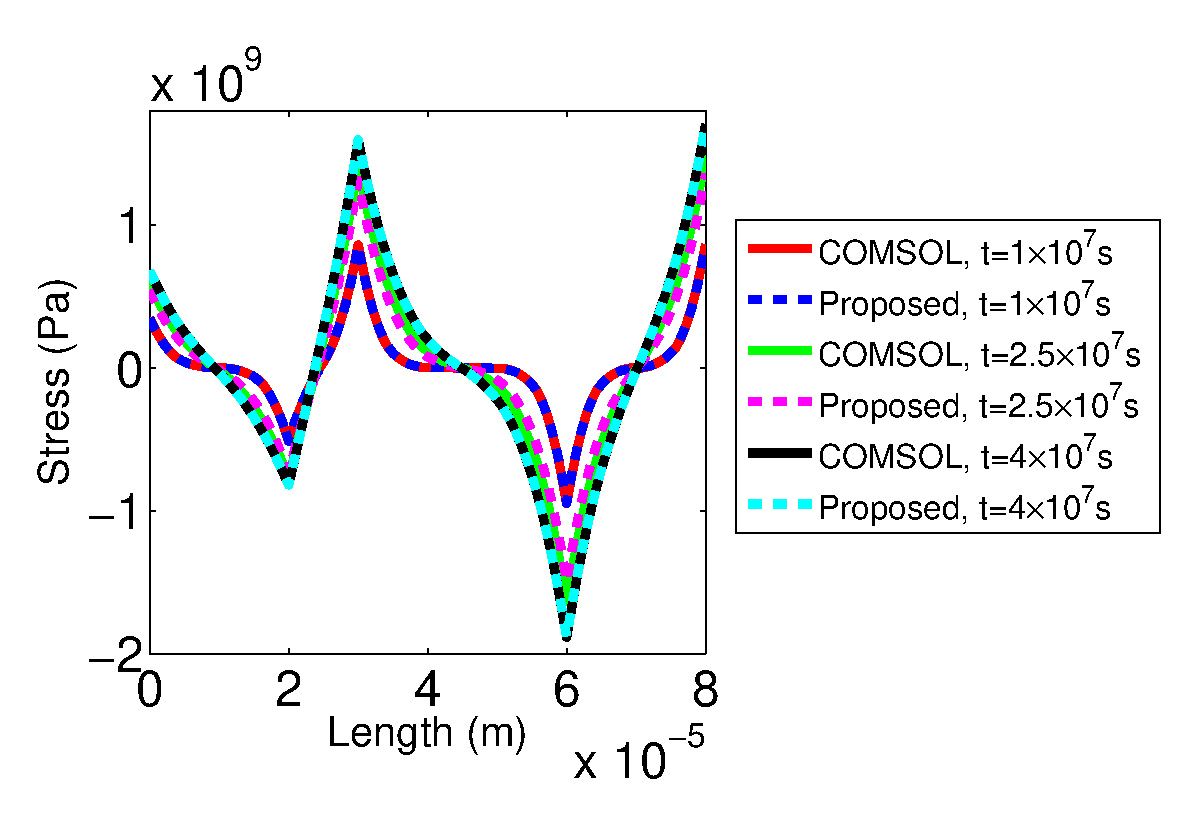
\includegraphics[width=0.9\columnwidth]{S4StressMatComCompareT0.eps}
\label{fig:ST4Compare}}
\subfigure[]{
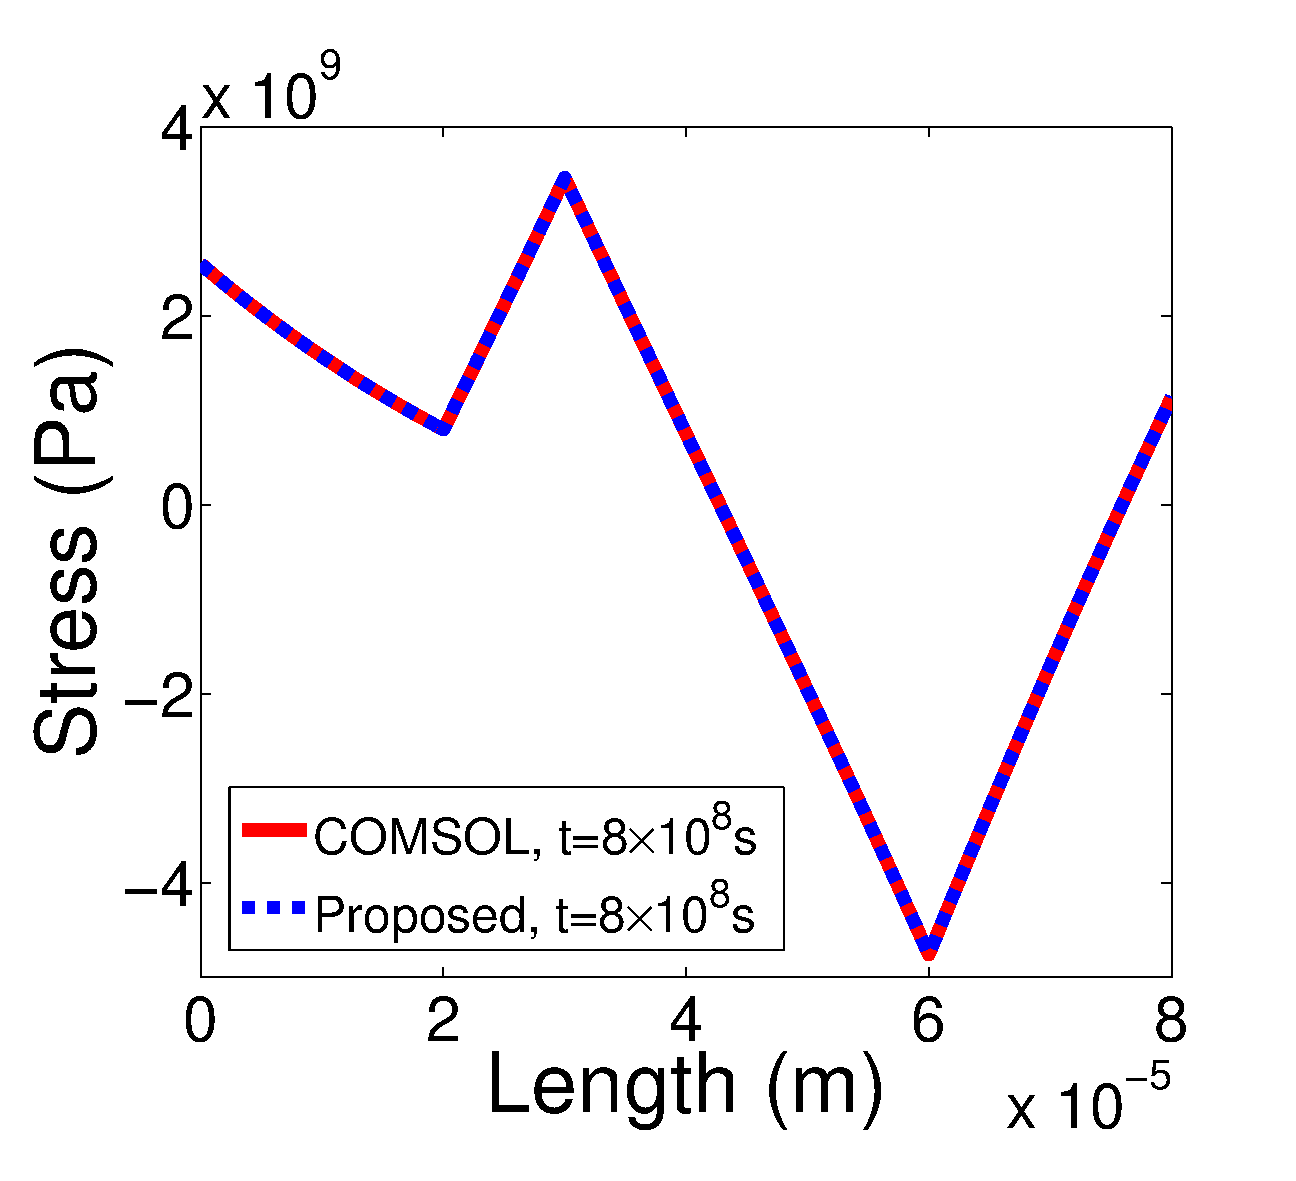
\includegraphics[width=0.6\columnwidth]{S4StableT0.eps}
\label{fig:ST4Stable}}
\caption{The experiments results of straight line at changing temperatures, $j_1=2\times10^{10}A/m^2,\;j_2=6\times10^{10}A/m^2$ (a) the comparison of stress evolution at square wave temperature at a fixed time; (b) the comparison of stress evolution at sine wave temperature at a fixed time; (c) the comparison of stress evolution at square wave temperature at a fixed position; (d) the comparison of stress evolution at sine wave temperature at a fixed position}
\label{fig:S4Results1}
\end{figure}


\begin{figure}[!h]
\centering
\subfigure[]{
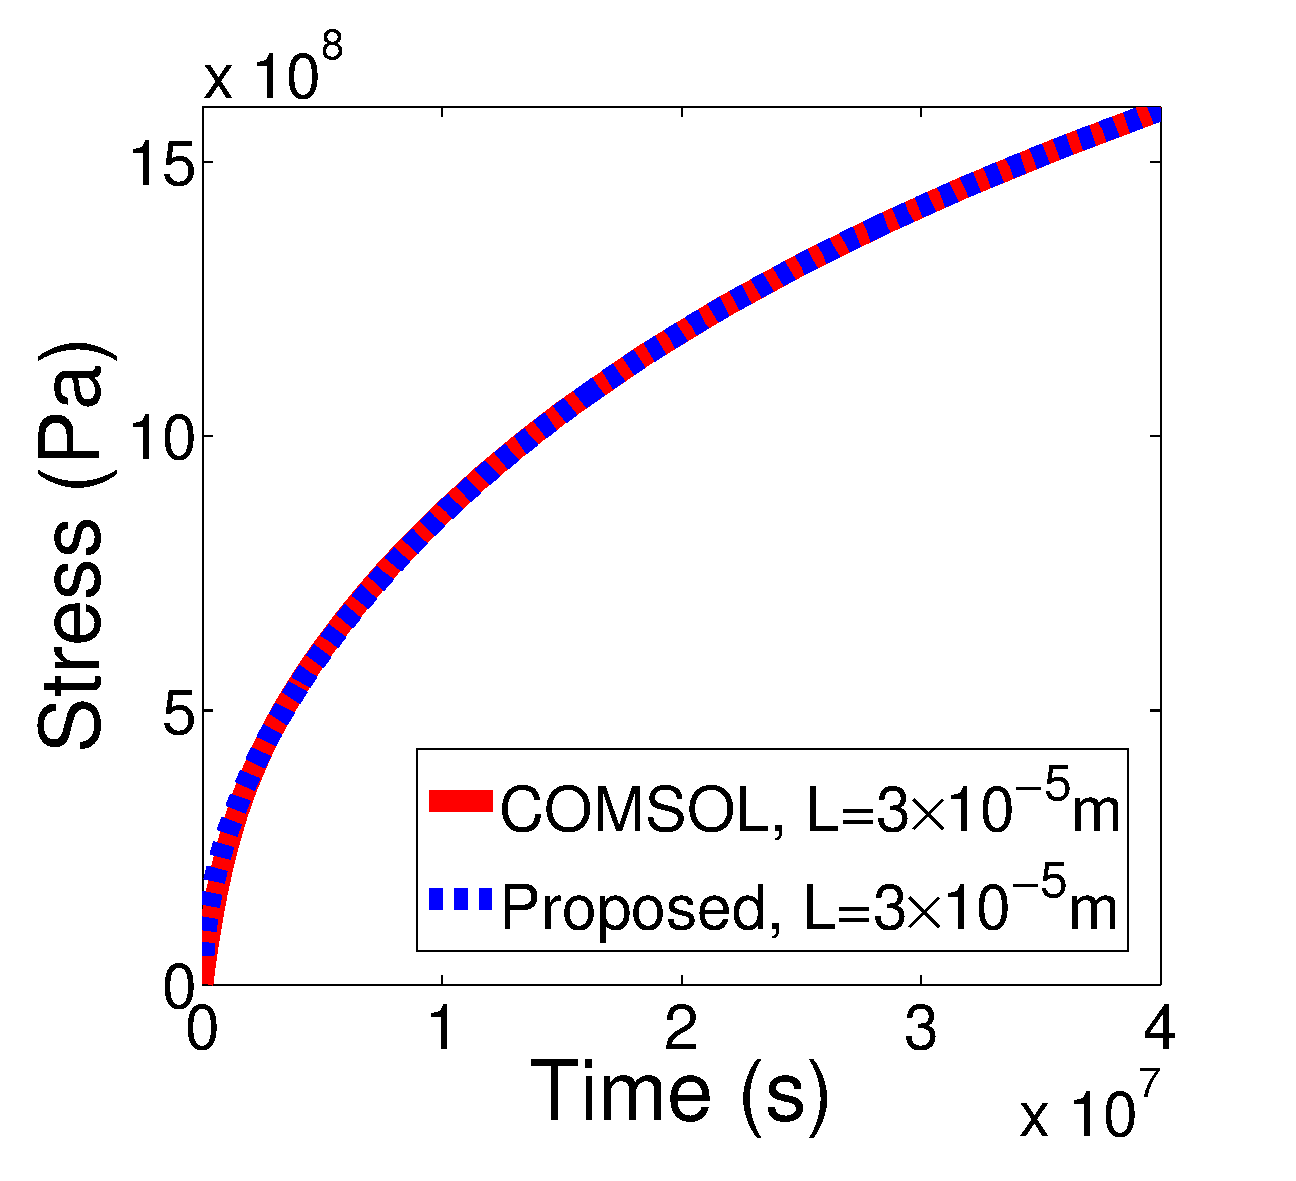
\includegraphics[width=0.45\columnwidth]{S4LengthCompare3T0.eps}
\label{fig:S4point1}}
\subfigure[]{
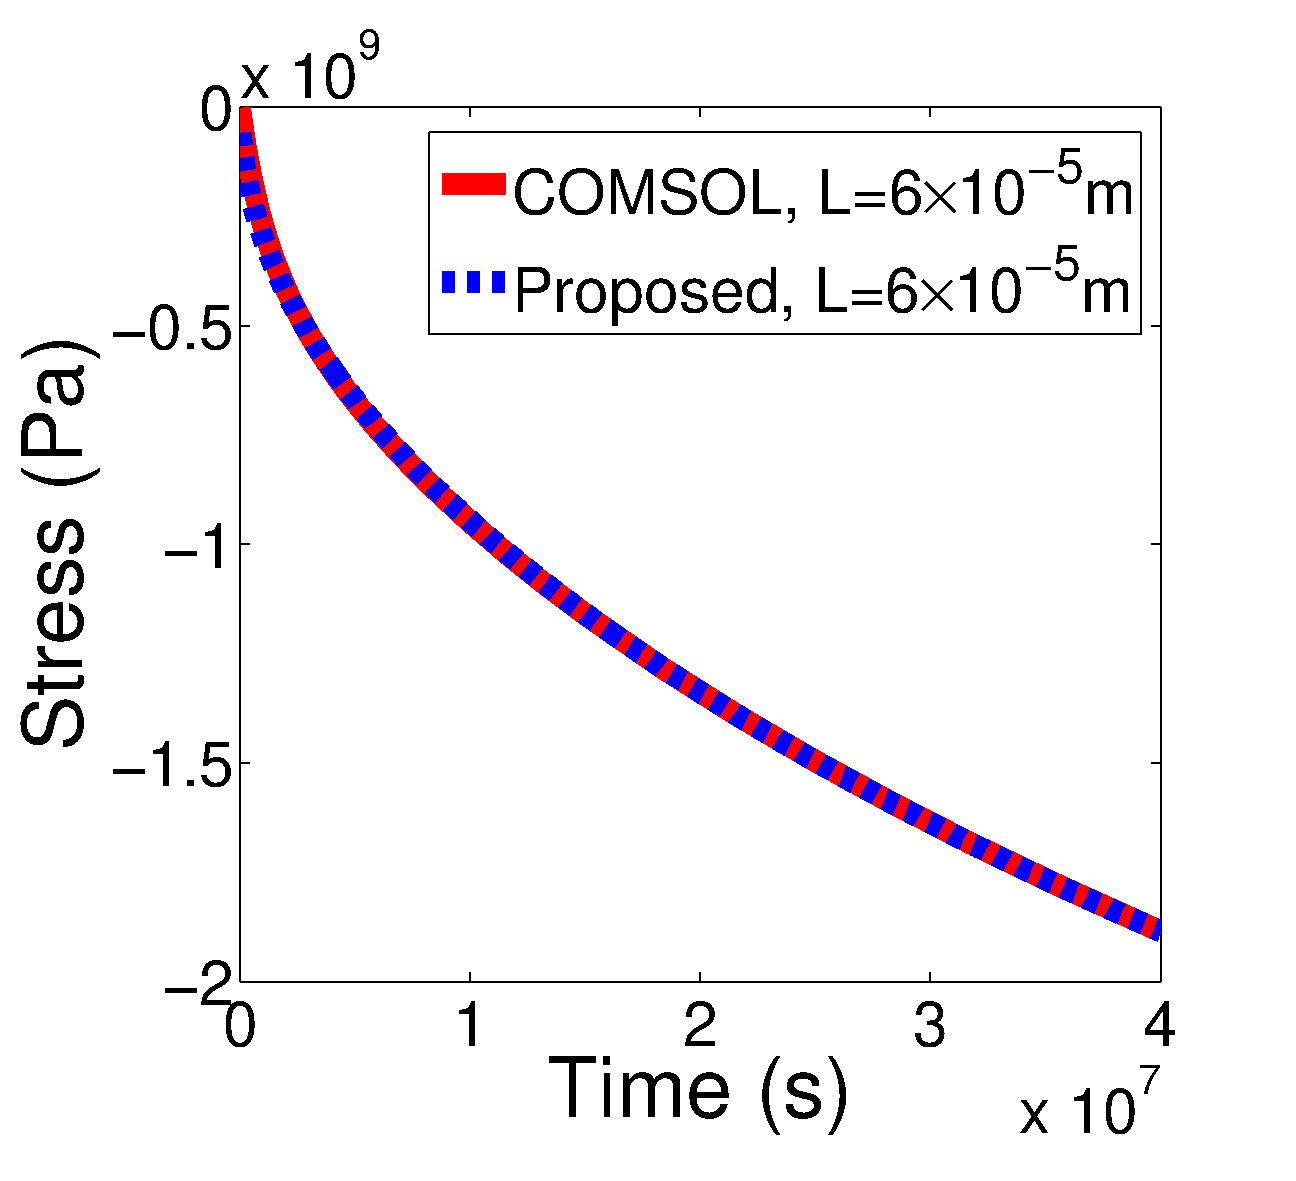
\includegraphics[width=0.45\columnwidth]{S4LengthCompare6T0.eps}
\label{fig:S4point2}}
\caption{The experiments results of straight line at changing temperatures, $j_1=2\times10^{10}A/m^2,\;j_2=6\times10^{10}A/m^2$ (a) the comparison of stress evolution at square wave temperature at a fixed time; (b) the comparison of stress evolution at sine wave temperature at a fixed time; (c) the comparison of stress evolution at square wave temperature at a fixed position; (d) the comparison of stress evolution at sine wave temperature at a fixed position}
\label{fig:S4Results2}
\end{figure}


\subsection{Six-terminal interconnect wire ($n=5$)}
\begin{figure}[!h]
\centering
\subfigure[]{
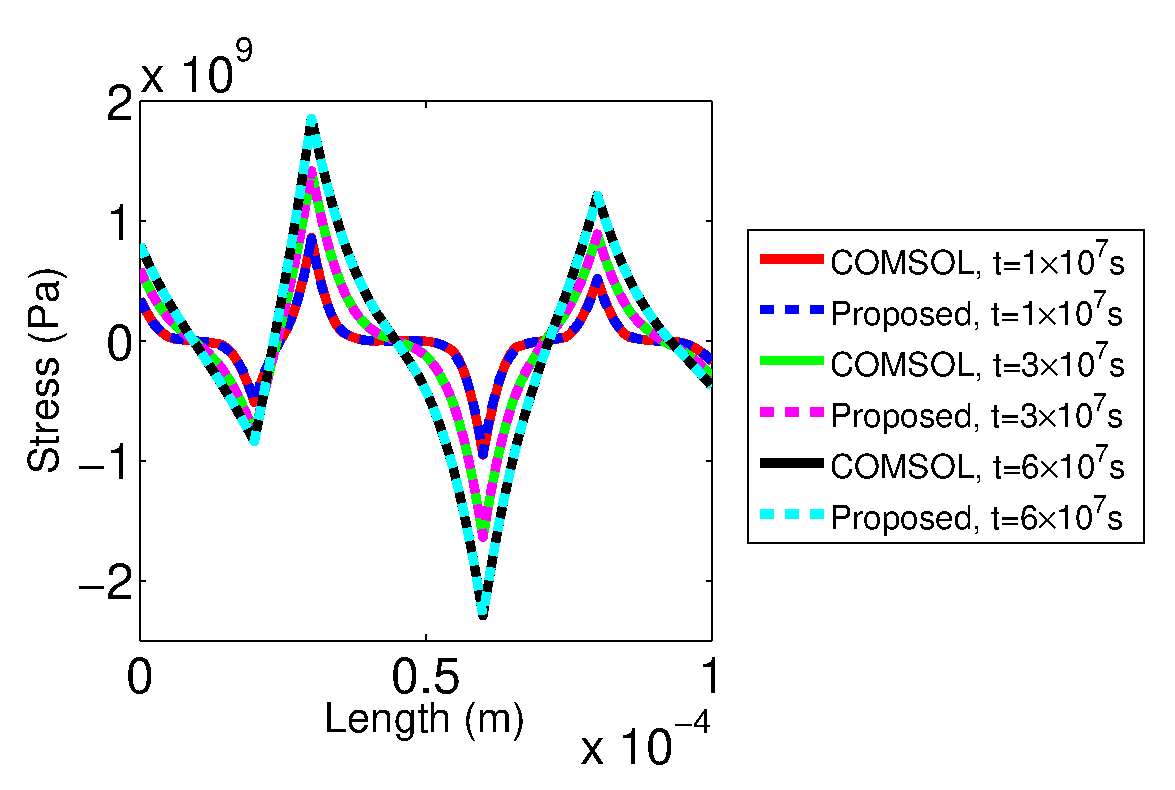
\includegraphics[width=0.9\columnwidth]{S5StressMatComCompareT0.eps}
\label{fig:ST5Compare}}
\subfigure[]{
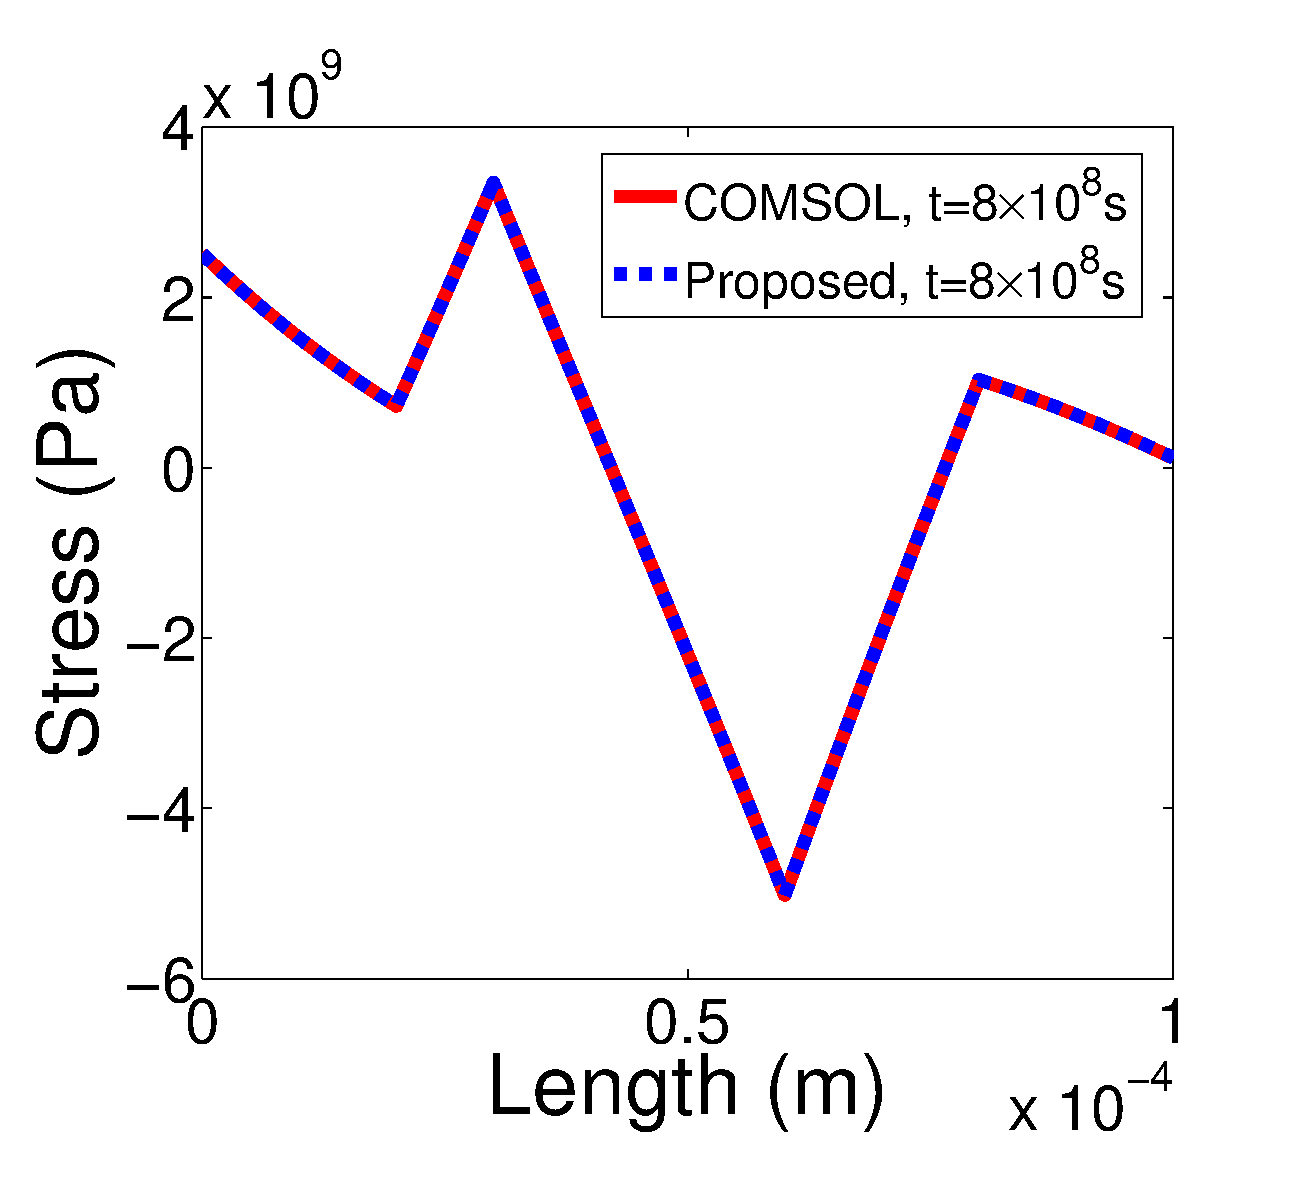
\includegraphics[width=0.6\columnwidth]{S5StableT0.eps}
\label{fig:ST5Stable}}
\caption{the}
\label{fig:S3Results1}
\end{figure}


\begin{figure}[!h]
\centering
\subfigure[]{
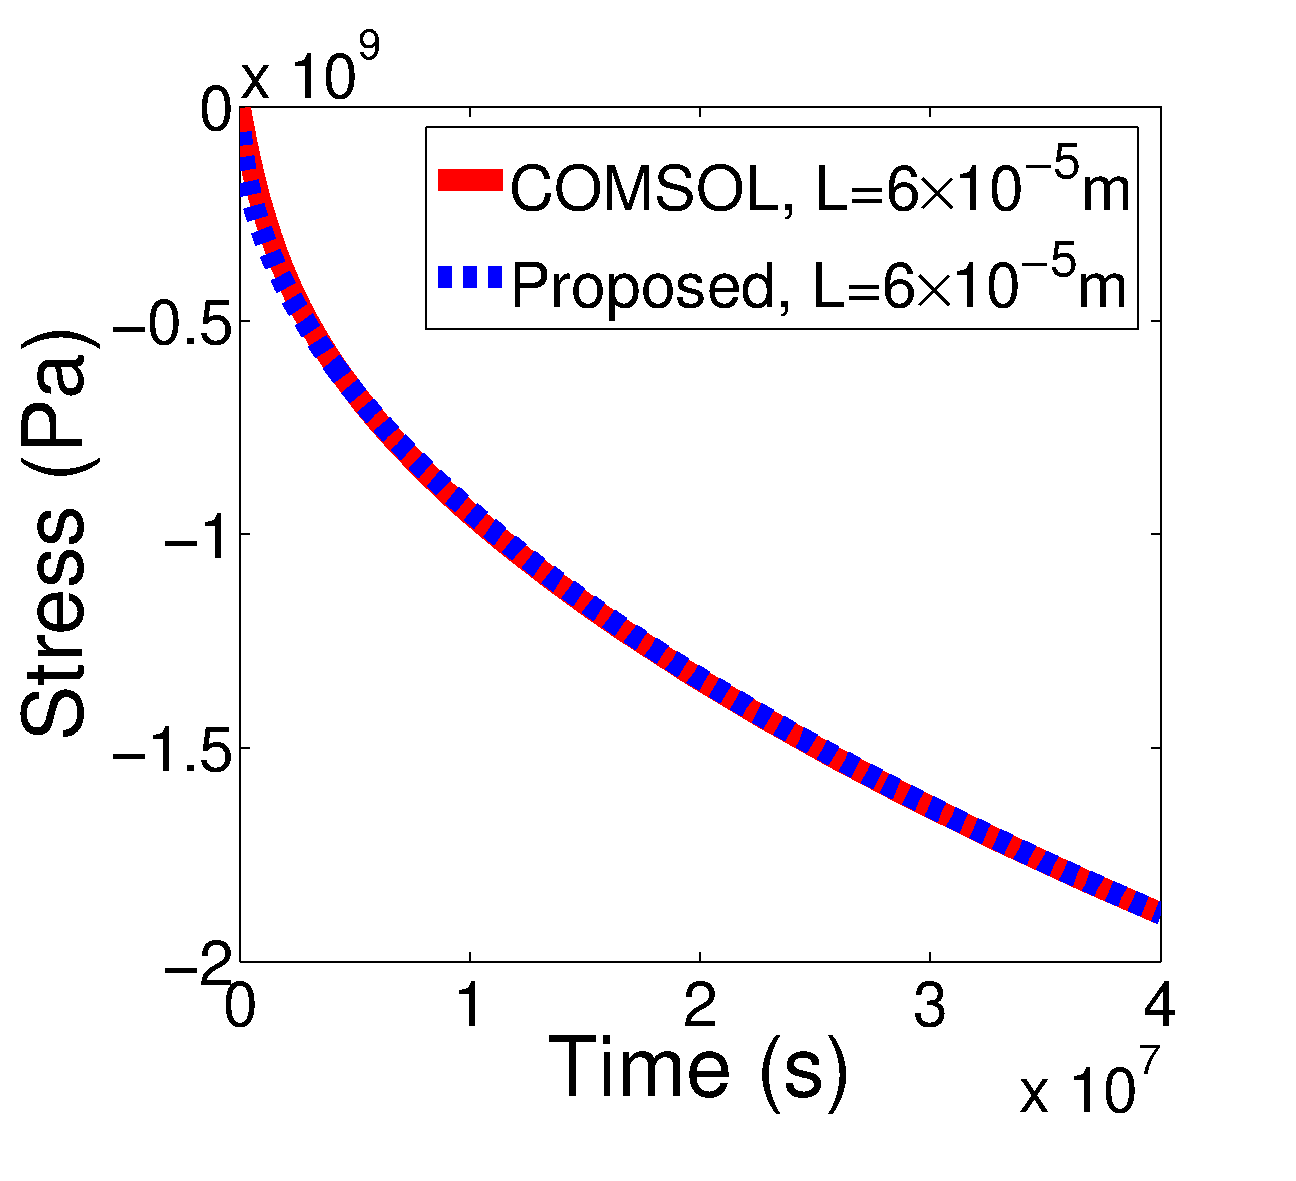
\includegraphics[width=0.45\columnwidth]{S5LengthCompare6T0.eps}
\label{fig:S5point1}}
\subfigure[]{
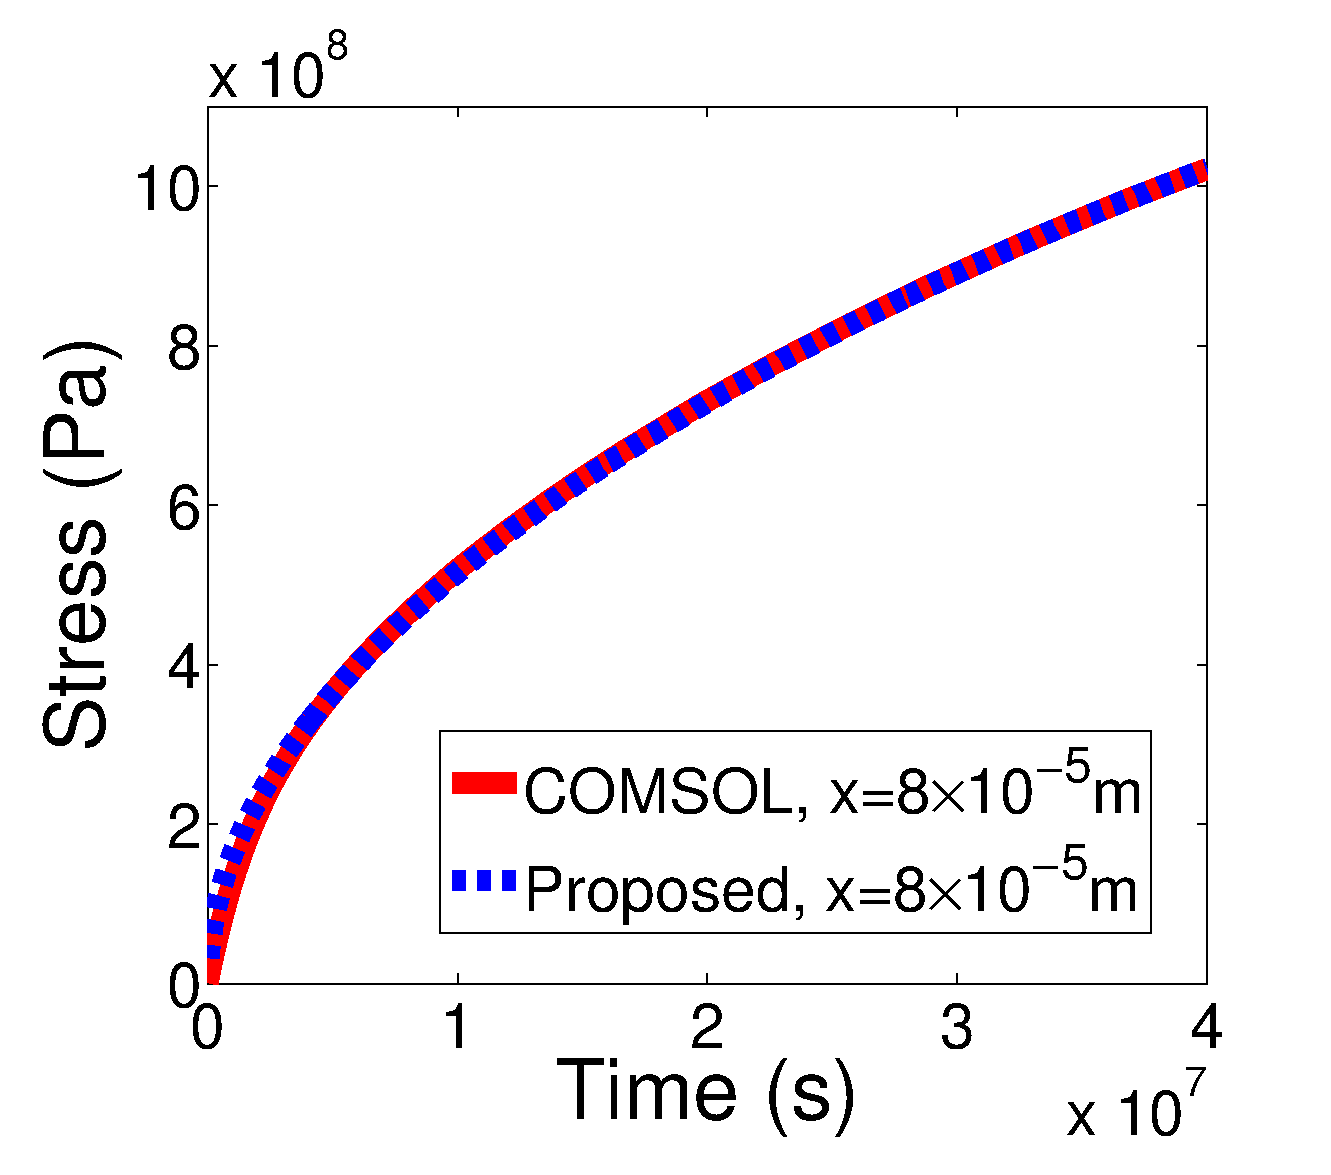
\includegraphics[width=0.45\columnwidth]{S5LengthCompare8T0.eps}
\label{fig:S5point2}}
\caption{The experiments results of straight line at changing temperatures, $j_1=2\times10^{10}A/m^2,\;j_2=6\times10^{10}A/m^2$ (a) the comparison of stress evolution at square wave temperature at a fixed time; (b) the comparison of stress evolution at sine wave temperature at a fixed time; (c) the comparison of stress evolution at square wave temperature at a fixed position; (d) the comparison of stress evolution at sine wave temperature at a fixed position}
\label{fig:S5Results2}
\end{figure}






%\subsection{T-shaped interconnect tree results}
%As expected in Fig.\ref{fig:TResults}, the stress distribution in the T-shaped tree shown in Fig.\ref{fig:Tshaped}, based on proposed analytical solution, has synchronized movement with numerical simulation in COMSOL. From Fig.\ref{fig:TT1Length} and Fig.\ref{fig:TT2Length},when the T-shaped tree works over $1\times10^{7}s$ in branch $1$, the stress as mild changes. So we just take two time values in Fig.\ref{fig:TT1Compare} and
%\begin{figure}[!h]
%\centering
%\subfigure[]{
%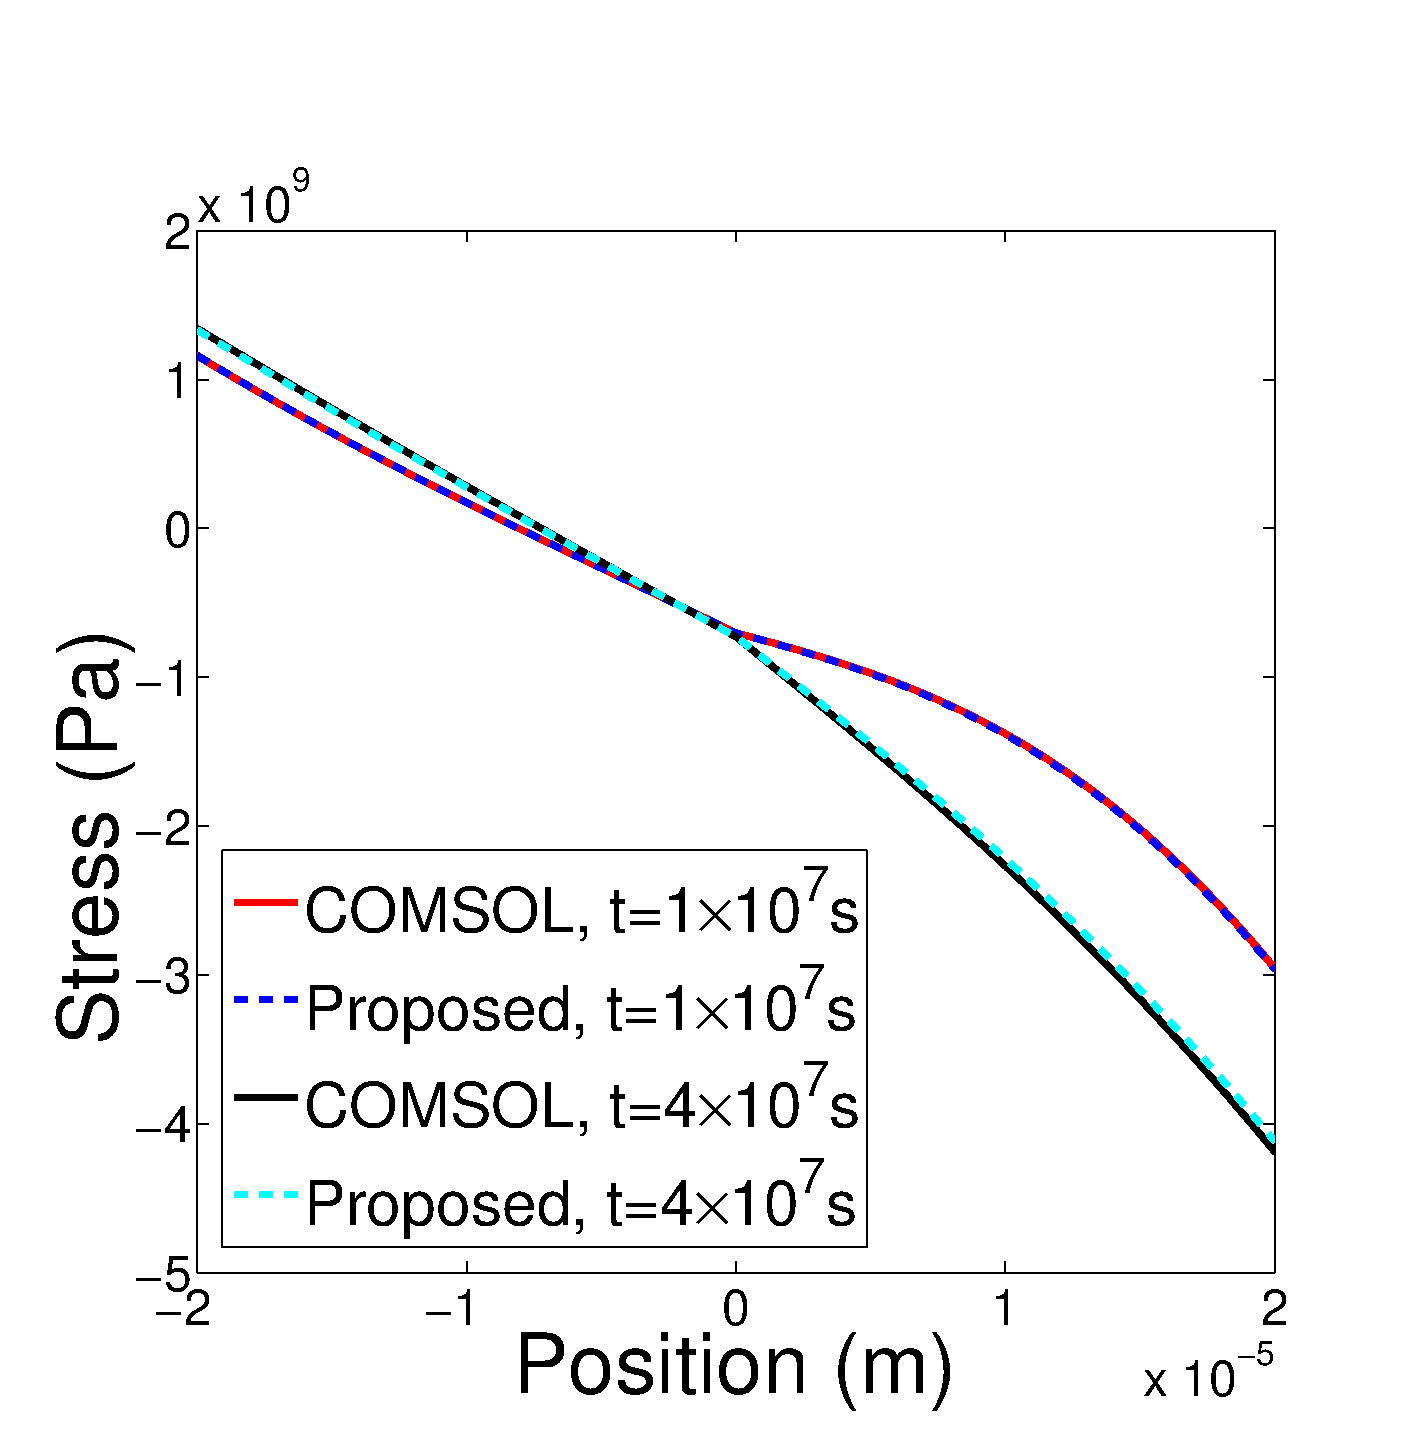
\includegraphics[width=0.45\columnwidth]{TStressMatComCompareT1.eps}
%\label{fig:TT1Compare}}
%\subfigure[]{
%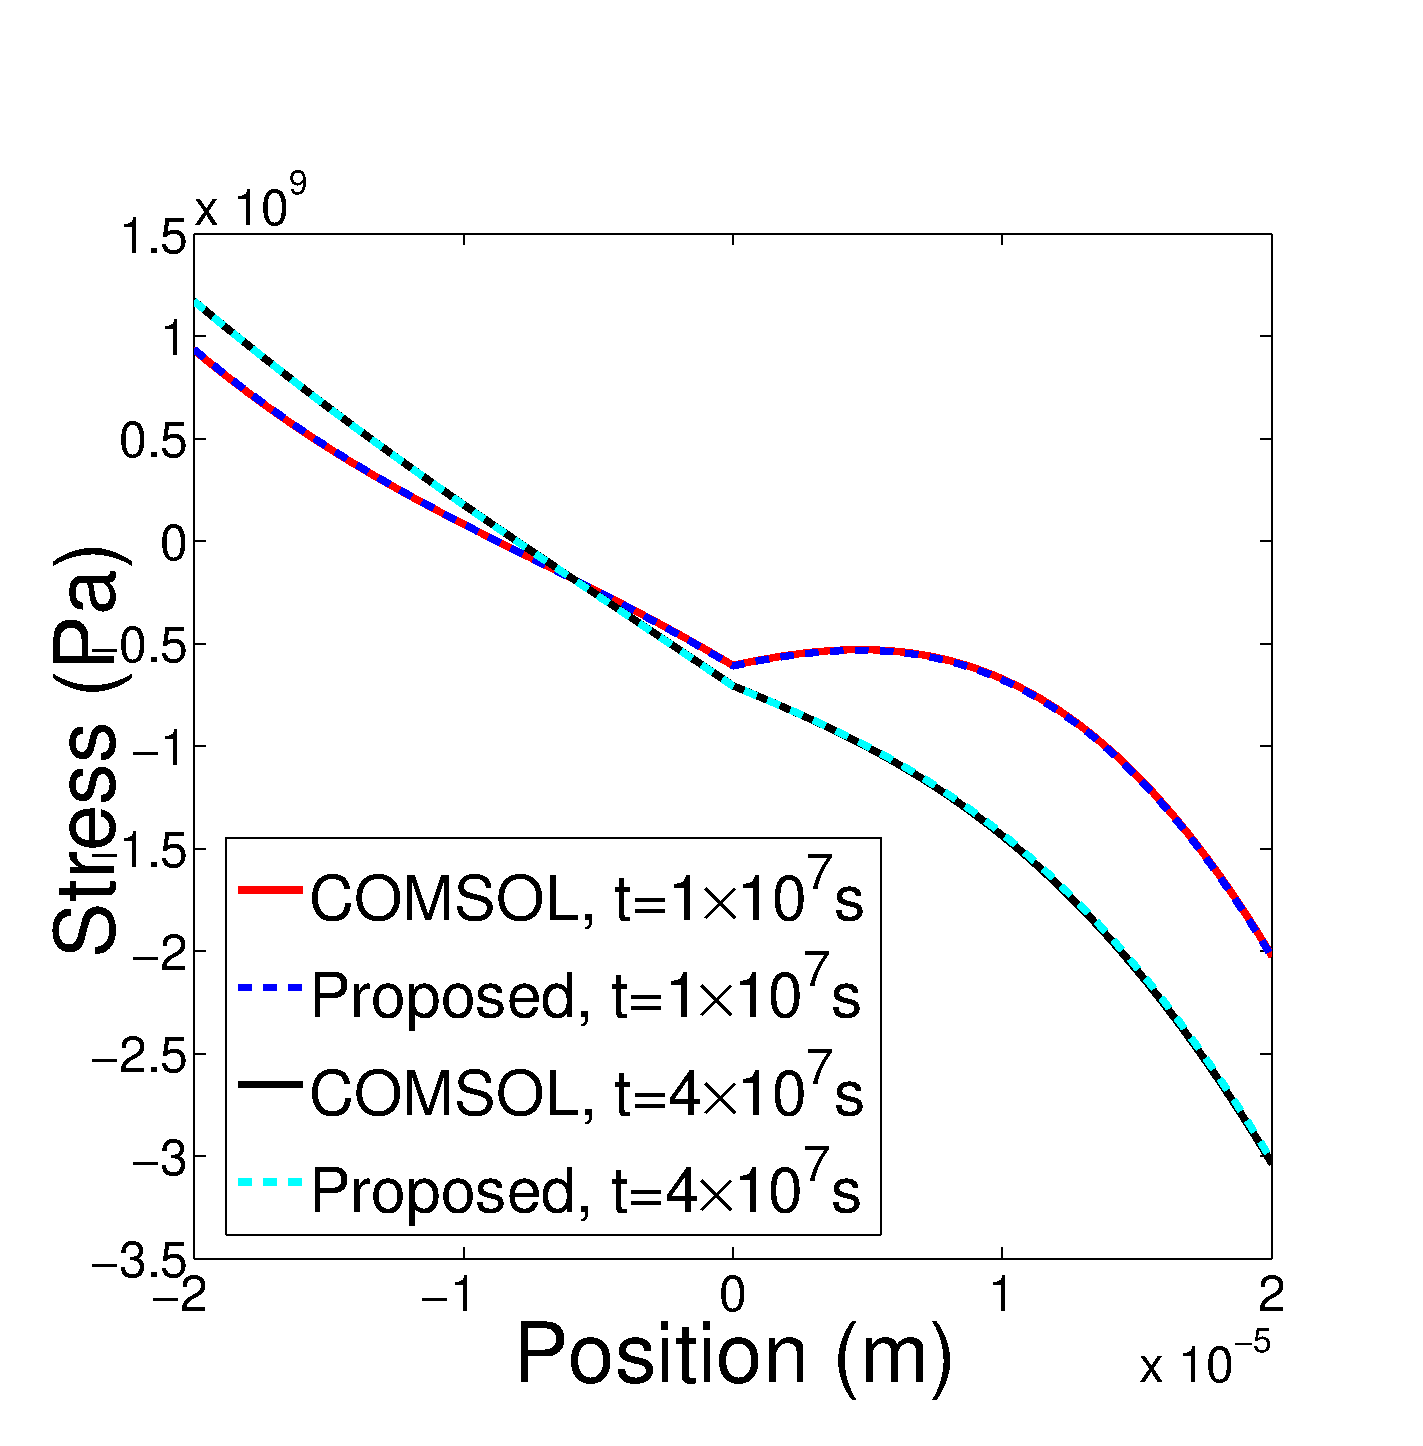
\includegraphics[width=0.45\columnwidth]{TStressMatComCompareT2.eps}
%\label{fig:TT2Compare}}
%\subfigure[]{
%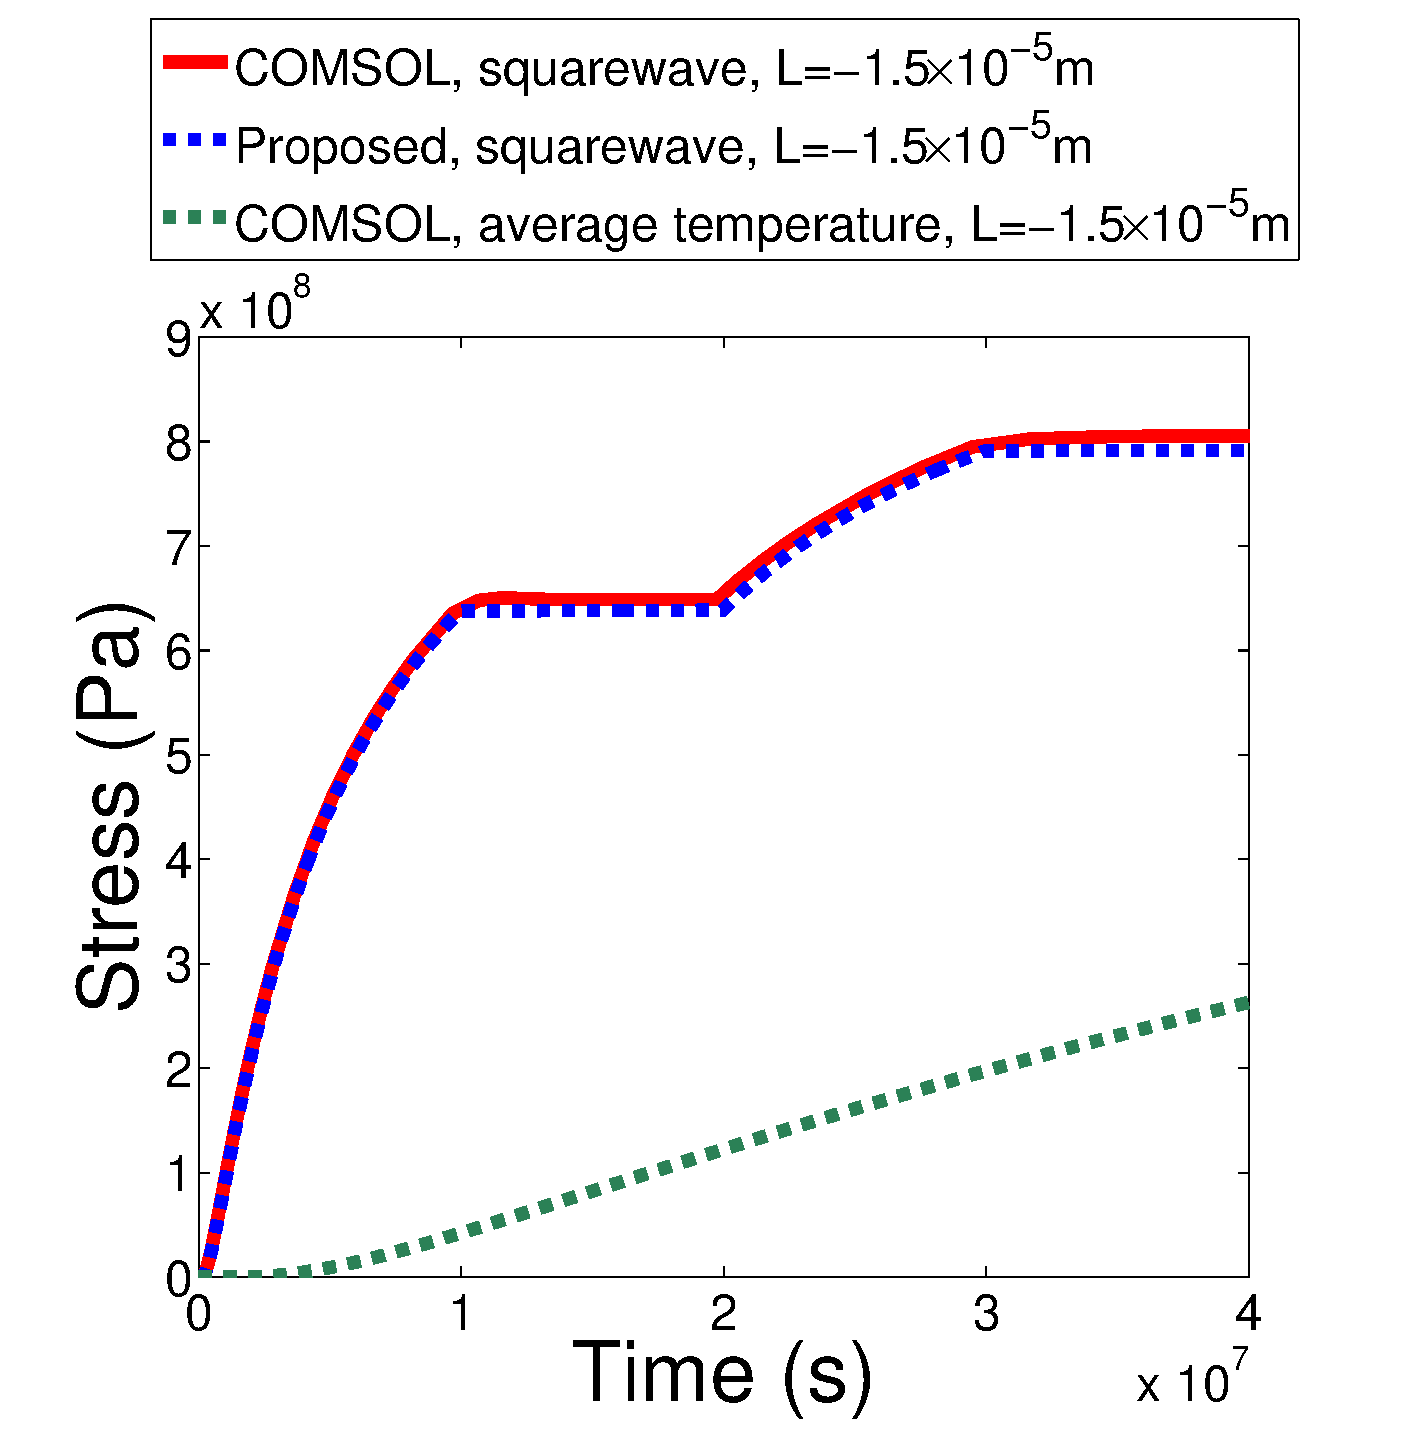
\includegraphics[width=0.45\columnwidth]{TLengthCompareT1.eps}
%\label{fig:TT1Length}}
%\subfigure[]{
%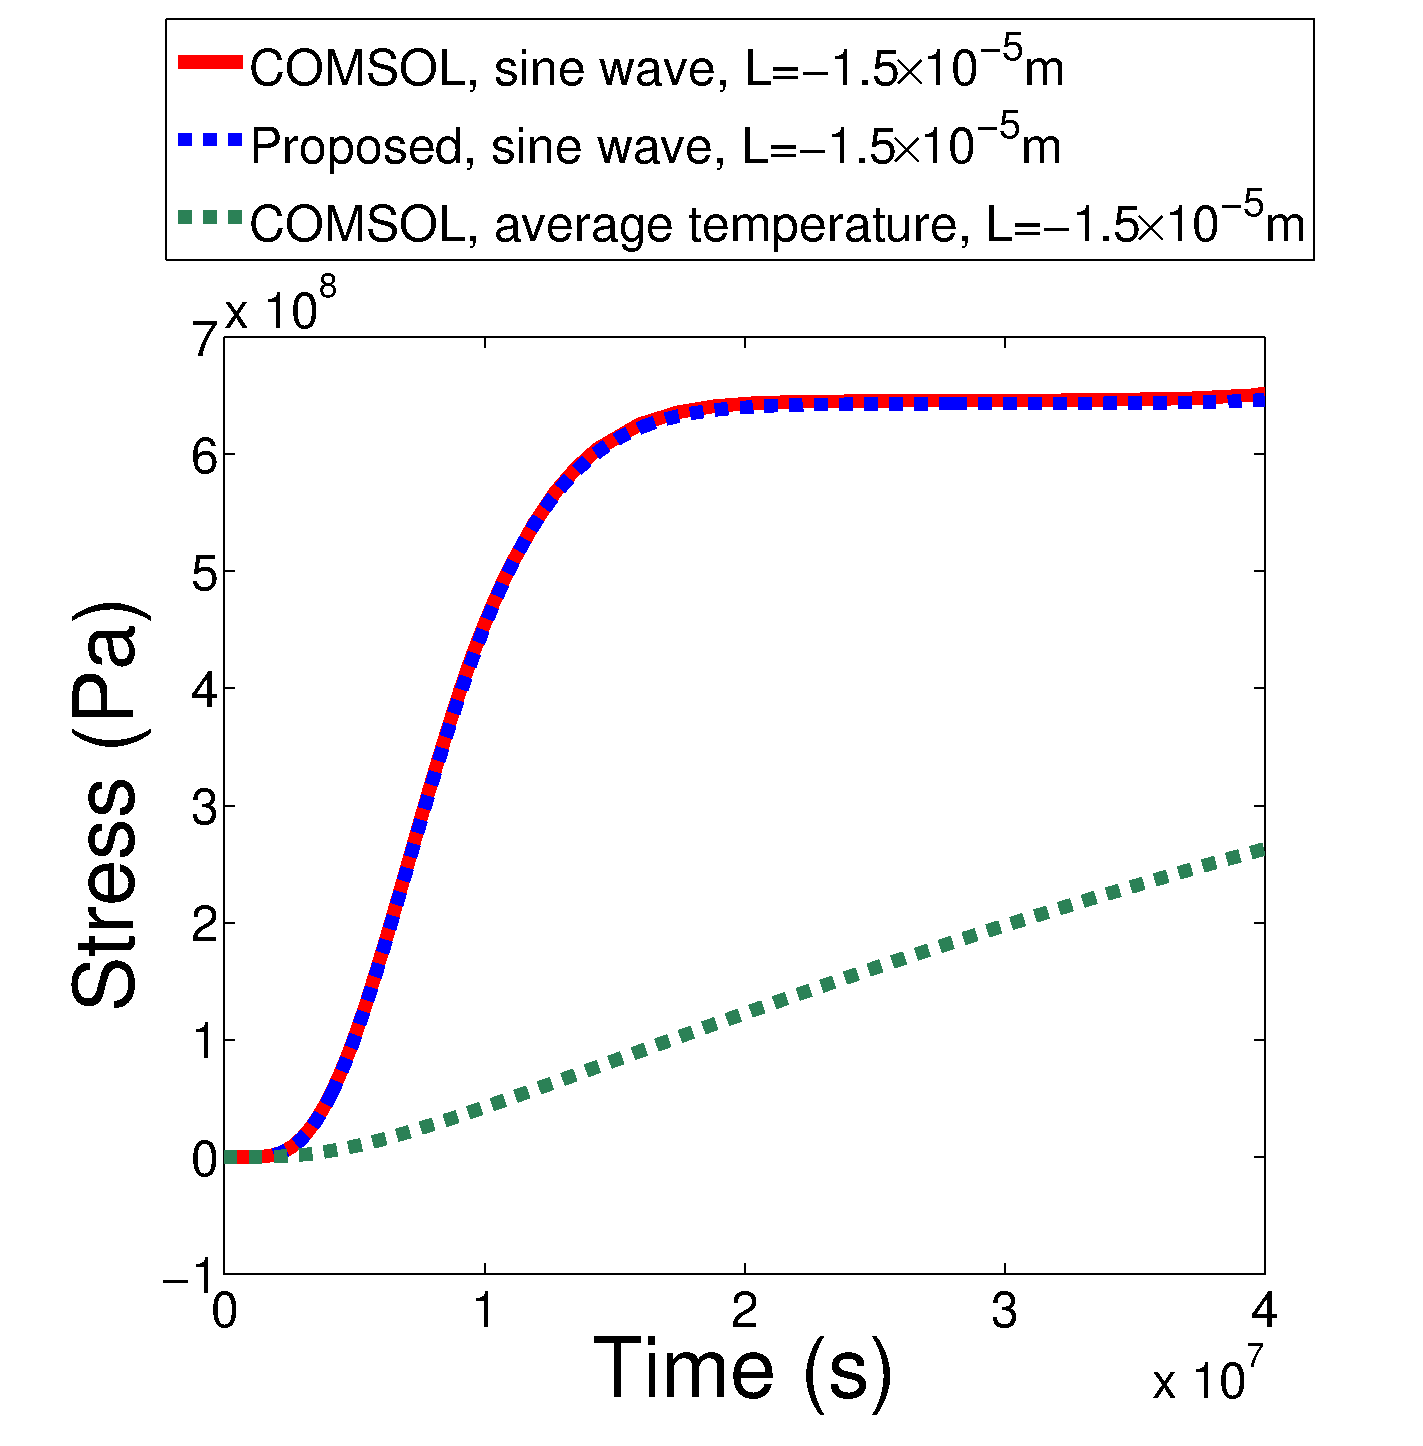
\includegraphics[width=0.45\columnwidth]{TLengthCompareT2.eps}
%\label{fig:TT2Length}}
%\caption{The experiments results of T-shaped interconnect tree at changing temperatures, $j_1=2\times10^{10}A/m^2,\;j_2=4\times10^{10}A/m^2,\;j_3=6\times10^{10}A/m^2$ (a) the comparison of stress evolution at square wave temperature at a fixed time; (b) the comparison of stress evolution at sine wave temperature at a fixed time; (c) the comparison of stress evolution at square wave temperature at a fixed position; (d) the comparison of stress evolution at sine wave temperature at a fixed position}
%\label{fig:TResults}
%\end{figure}
%
%\subsection{Cross-shaped interconnect tree results}
%From Fig.\ref{fig:CResults} considering the basic tree shown in Fig.\ref{fig:Cshaped}, we can see that the stress evolution of proposed model fits well to those obtained from COMSOL. Without the proposed model, we maybe use the average temperature to estimate the stress evolution.
%\begin{figure}[!h]
%\centering
%\subfigure[]{
%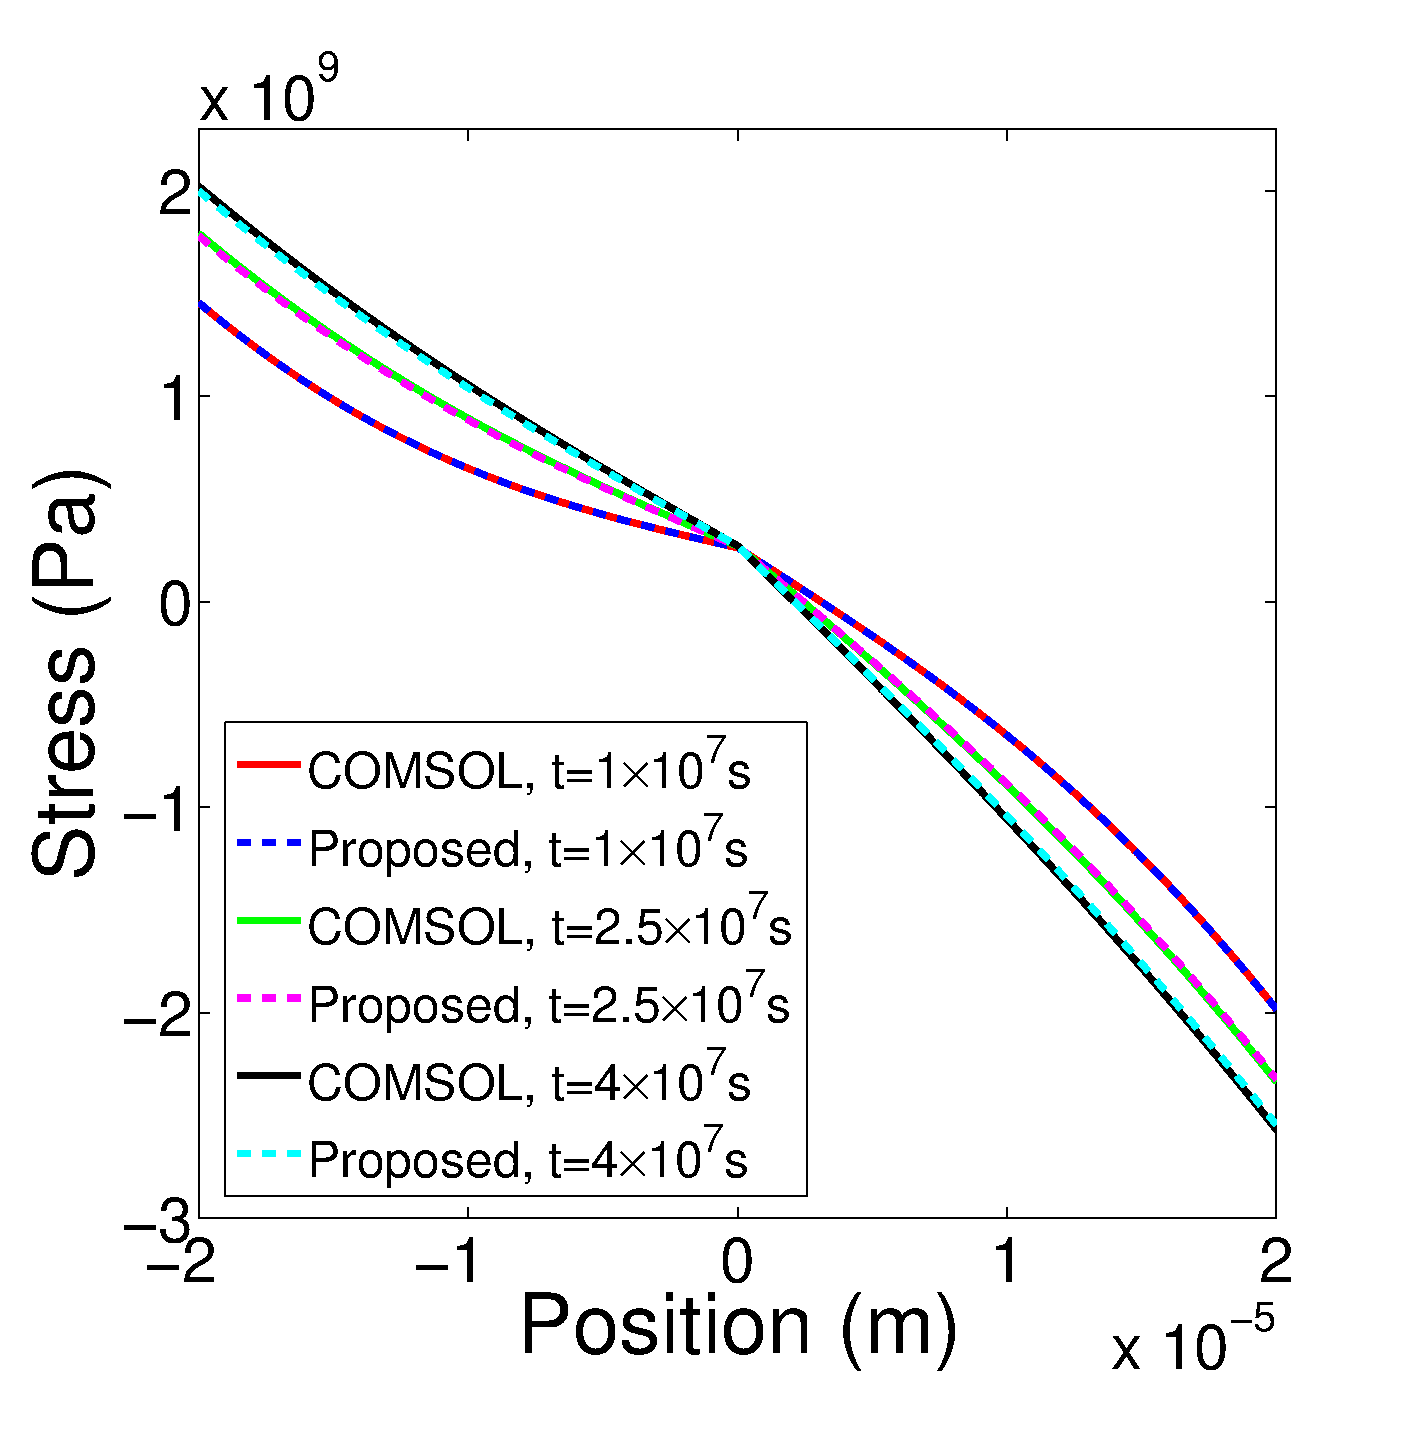
\includegraphics[width=0.45\columnwidth]{CStressMatComCompareT1.eps}
%\label{fig:CT1Compare}}
%\subfigure[]{
%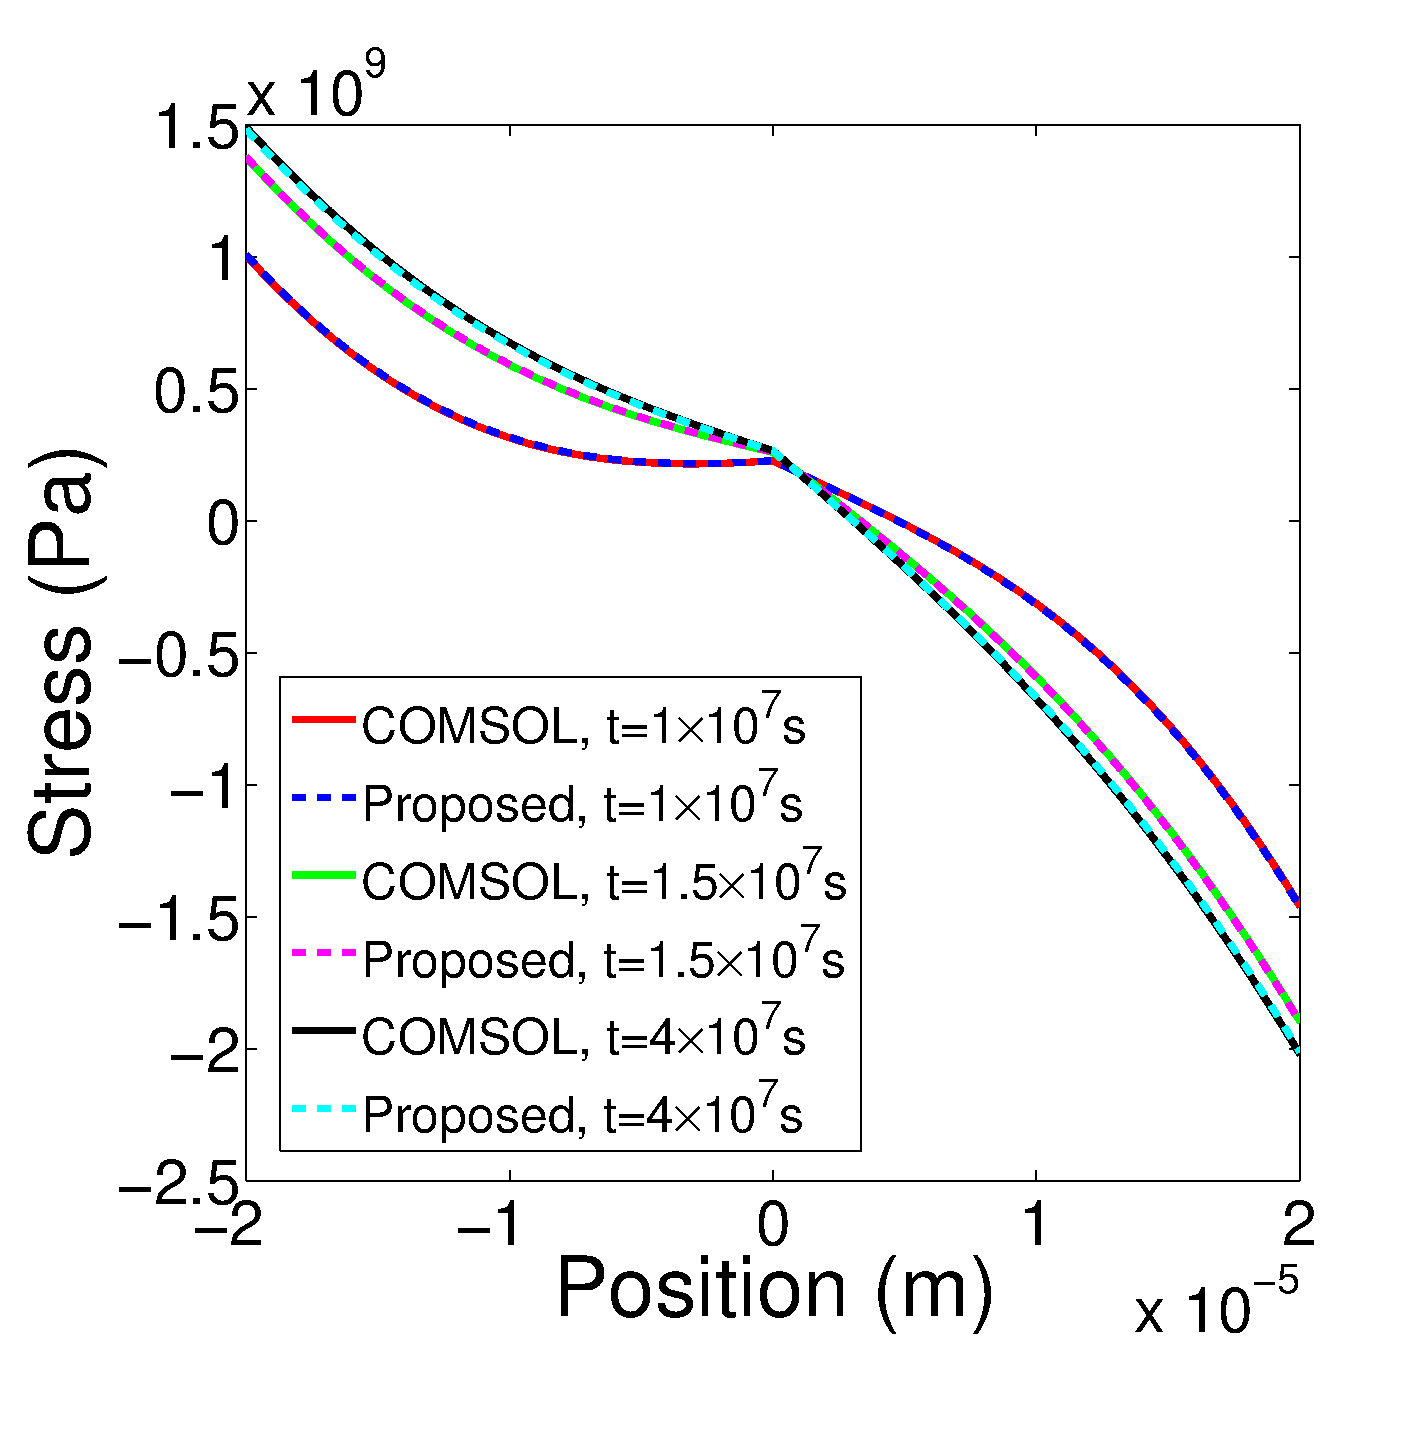
\includegraphics[width=0.45\columnwidth]{CStressMatComCompareT2.eps}
%\label{fig:CT2Compare}}
%\subfigure[]{
%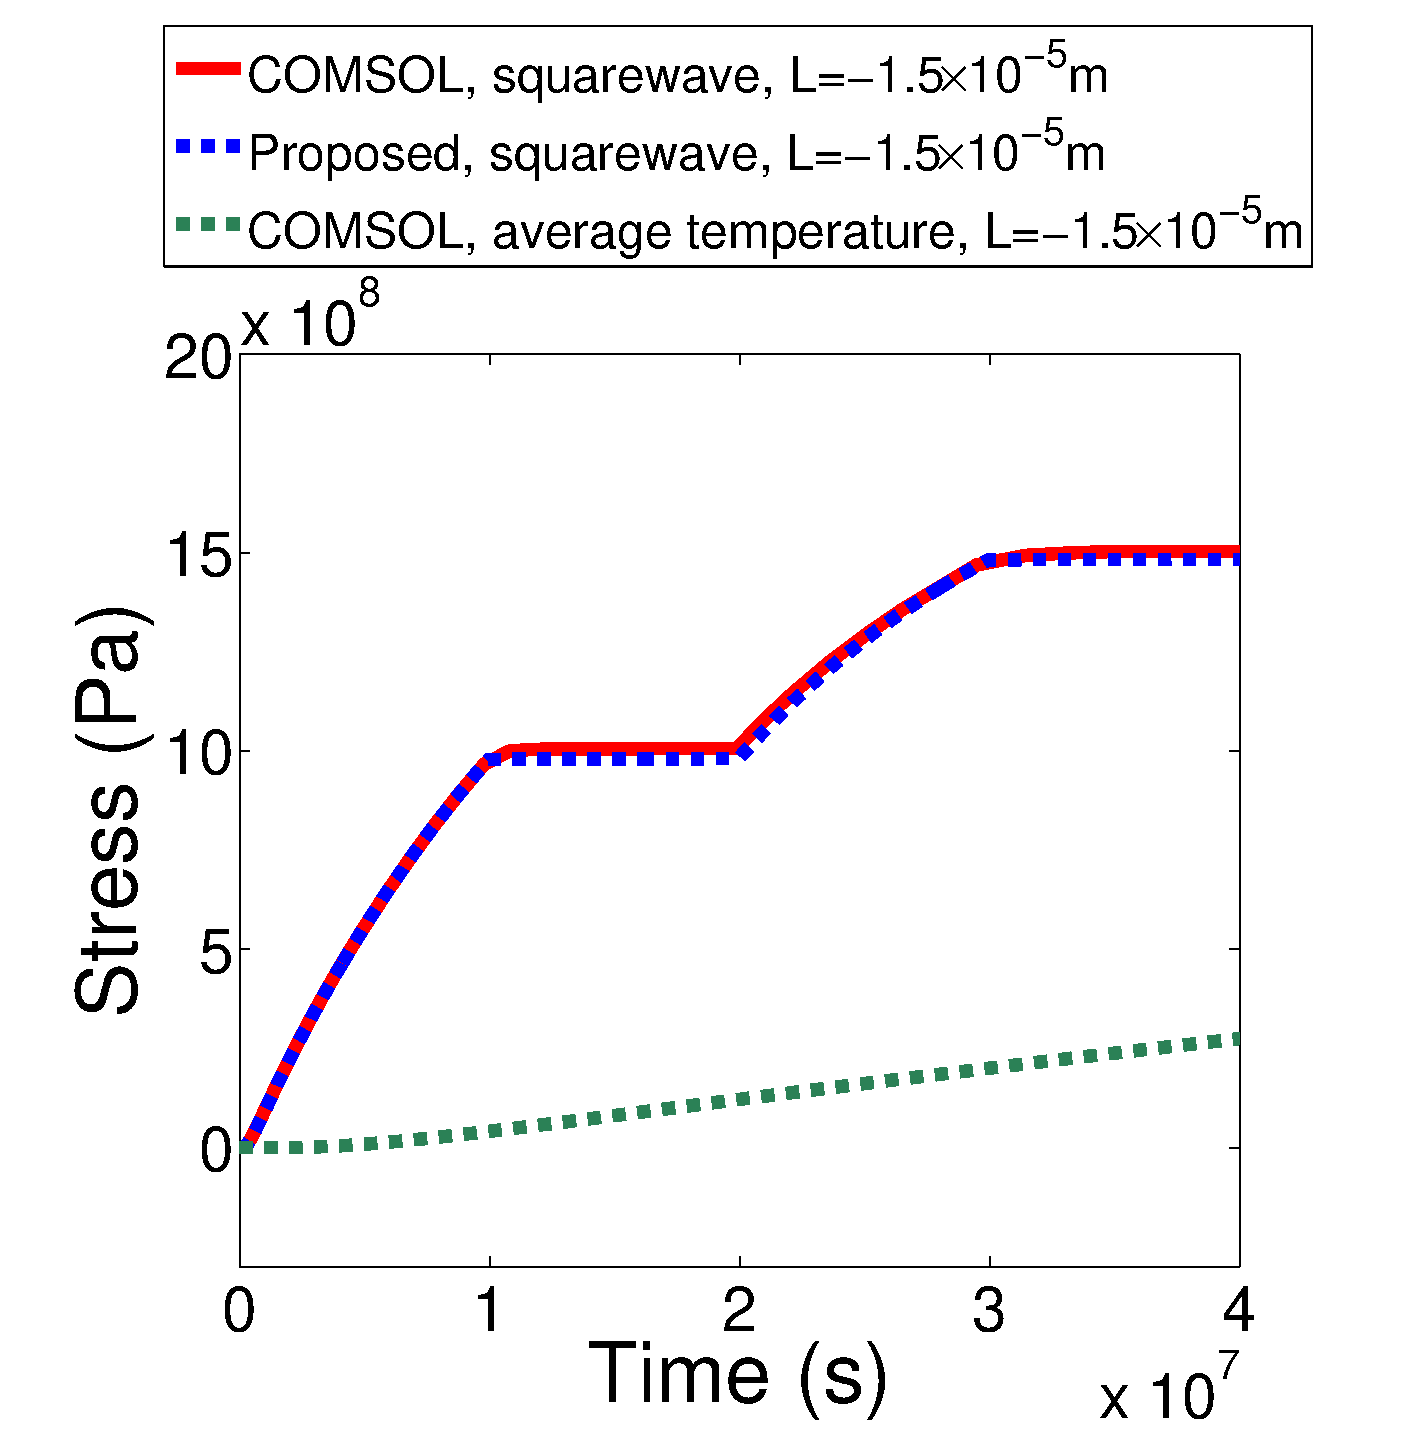
\includegraphics[width=0.45\columnwidth]{CLengthCompareT1.eps}
%\label{fig:CT1Length}}
%\subfigure[]{
%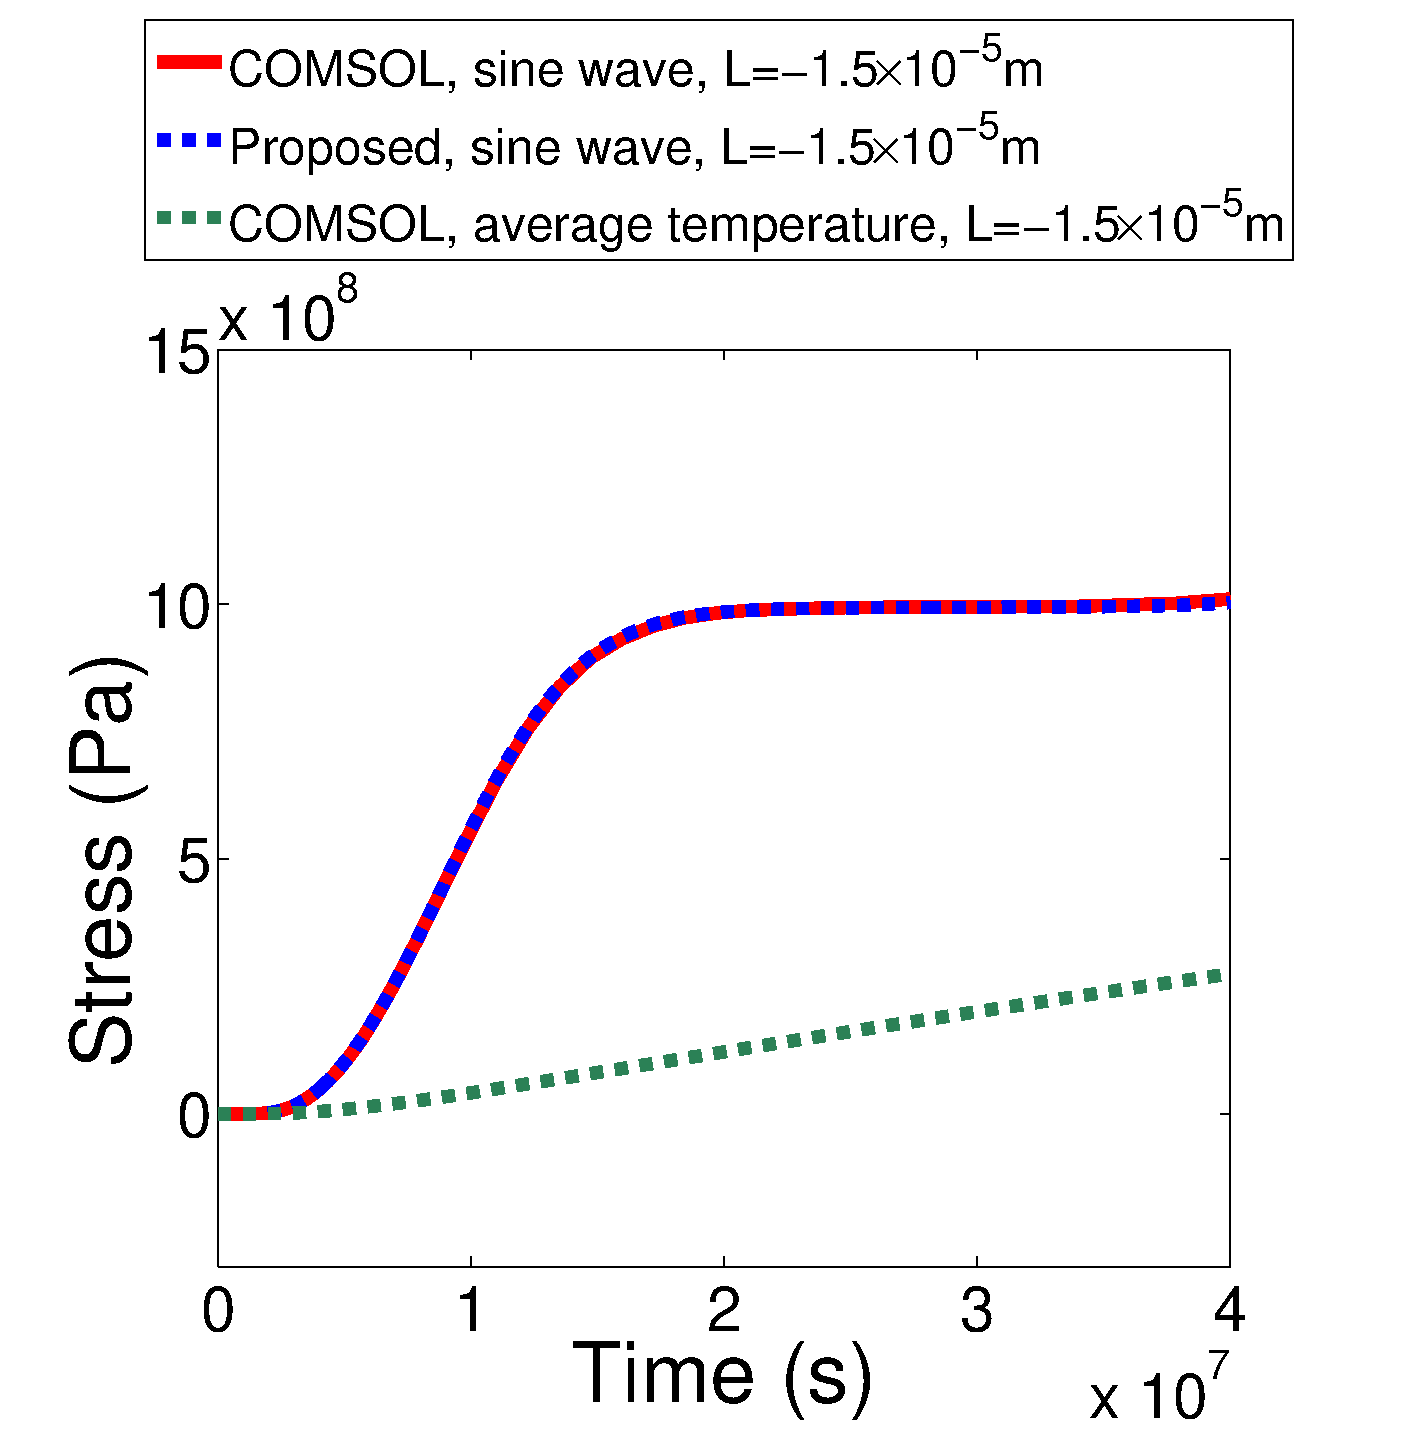
\includegraphics[width=0.45\columnwidth]{CLengthCompareT2.eps}
%\label{fig:CT2Length}}
%\caption{The experiments results of T-shaped interconnect tree at changing temperatures, $j_1=2\times10^{10}A/m^2,\;j_2=3\times10^{10}A/m^2,\;j_3=4\times10^{10}A/m^2,\;
%j_4=5\times10^{10}A/m^2$ (a) the comparison of stress evolution at square wave temperature at a fixed time; (b) the comparison of stress evolution at sine wave temperature at a fixed time; (c) the comparison of stress evolution at square wave temperature at a fixed position; (d) the comparison of stress evolution at sine wave temperature at a fixed position}
%\label{fig:CResults}
%\end{figure}
